\providecommand{\main}{../..}  % define path to bib location for subfiles
\documentclass[../../main.tex]{subfiles}
\begin{document}
\onlyinsubfile{
%\setcounter{chapter}{8}
}
\notinsubfile{}
\chapter{Docentenhandleiding}

\section{De module in een oogopslag}\label{chap:Hoog}
%\marginpar{\nogdoen{module-cie moet dit hier of in docentenhandleiding? Tekst is gekopi\"eerd uit par 1.1}}
In deze module maak je kennis met quantumcomputing. De module bestaat uit twee delen. In het eerste deel bouwen we ons begrippenapparaat op, in het tweede deel passen we onze kennis toe in praktische opdrachten. Het eerste deel bestaat uit drie hoofdstukken. Alle hoofdstukken hebben een aantal werkbladen. In hoofdstuk~\ref{chap:H1} beginnen we met een korte inleiding op het onderwerp en maken we kennis met enkele belangrijke begrippen en fenomenen door zelf te experimenteren met licht. Om de vergelijking te maken met een quantumcomputer begint hoofdstuk~\ref{chap:H2} met een korte uitleg over hoe een klassieke computer werkt. We onderbouwen ons wiskundig begrippenapparaat met een model. Het hoofdstuk eindigt met een eisenlijst waaraan een quantumcomputer moet voldoen. In ~\ref{chap:H3} behandelen we de bouwblokken (poorten) van quantumcomputers. We zien dat die echt anders zijn. We leren hiermee werken en het hoofdstuk sluit af met een protocol waar alle eigenschappen van een quantumcomputer in voorkomen: teleportatie. Na dit hoofdstuk volgt een toets. \\
Het tweede deel (hoofdstuk~\ref{chap:H4}) is een verzameling praktische keuze-opdrachten. Daarin leer je pas goed hoe de quantumcomputer is toe te passen. Je onderzoekt in samenwerkingsverband een aspect van quantumcomputing; een algoritme, een verdieping in wiskunde D, een technisch of een maatschappelijk aspect. Er is ook de mogelijkheid om dit deel in te vullen met een activiteit aangeboden door een van de universiteiten. 
\iffalse
het tweede deel bestaat uit keuzeopdrachten waarvoor je in de lessen aanwijzingen krijgt. In hoofdstuk~\ref{chap:H4} werken we met quantumalgoritmen. Met spelletjes maken we nog eens duidelijk dat een quantumcomputer echt andere dingen kan dan een klassieke computer. Hoofdstuk~\ref{chap:H5} behandelt hoe je een quantumcomputer bouwt. Hoofdstuk~\ref{chap:H6} schetst aan de hand van enkele concrete voorbeelden welke problemen quantumcomputers een rol kunnen spelen in de maatschappij en we speculeren we voorzichtig over de toekomst. Na hoofdstuk zes volgen nog verdiepingsopdrachten voor wiskunde~D. In werkbladen staan enkele praktische opdrachten uitgewerkt. Een uitgebreide literatuurlijst met voornamelijk open access bronnen geeft je toegang tot oorspronkelijke literatuur. 
\fi
%\bigskip
\marginpar{\vspace{-4cm}
\includegraphics[width=0.95\marginparwidth]{./img/smartphone verplicht.png}
Tip: Voor de papieren versie zijn de links als QR-codes opgenomen. Gebruik je telefoon!}

Deze reader is het best te lezen in elektronisch (pdf) formaat. Voor de papieren versie zijn voor de links QR-codes in de marge opgenomen. We kunnen niet al ons materiaal in deze reader kwijt. In de docentenhandleiding en op de~\hrefqr[-1cm]{www.quantumrules.nl}{website} van het project staat meer ondersteunend materiaal.

%\bigskip
Veel plezier, De auteurs
\newpage

\subsection*{Doelgroep} De module is bedoeld voor een brede populatie van leerlingen eind 5~VWO of 6~VWO.
Het is mogelijk dat In een NLT-klas komen zowel leerlingen zitten die quantumfysica en de toepassing daarvan die in deze module wordt besproken zien als een vanzelfsprekend onderdeel van hun curriculum. Dit zullen leerlingen zijn die zeker natuurkunde en wiskunde-B in hun pakket hebben. Maar er zullen ook leerlingen zijn zonder natuurkunde en alleen wiskunde-A in hun pakket.  
Ook voor deze leerlingen is deze module bedoeld al was het maar om enig inzicht te verschaffen in het magische onderwerp quantumfysica dat zo vaak wordt genoemd in allerlei documenten. We proberen een boodschap over zin en onzin over deze technologie mee te geven. In ieder geval zullen alle leerlingen ondervinden dat een quantumcomputer echt anders is dan een klassieke computer.

\subsection*{Benodigde voorkennis}
Wat de wiskunde betreft is de meeste voorkennis die van 3 VWO.  De taal van quantumcomputing is lineaire algebra. Leerlingen moeten dan ook een lineaire combinatie kunnen herschrijven. Ze moeten vertrouwd zijn met het ‘werken met haakjes’. In deze module wordt geen gebruik gemaakt van de matrixrekening. Wel wordt gebruik gemaakt van het begrip vector dat bij het vak natuurkunde in 3~VWO wordt behandeld. De in de wiskunde gebruikelijke vectornotatie wordt in de tekst uitgelegd. 
Belangrijk is ook dat in de module veel wordt gewerkt met projecties van vectoren. Dat vereist elementaire kennis van de goniometrie. Bij natuurkunde komt dat in de vierde klas uitgebreid aan de orde. Voor alle leerlingen die natuurkunde in het pakket hebben is er dus geen enkel probleem. 
Leerlingen met wiskunde A en zonder natuurkunde zullen niet bekend zijn met projecties van vectoren (gonio). Een steunles voor deze leerlingen voorafgaand aan hoofdstuk~2 is hier op zijn plaats.

Wat de natuurkunde betreft is er voorkennis nodig van het verschijnsel trillingen en golven.  Met name het verschijnsel interferentie speelt in deze module een rol. Als leerlingen geen natuurkunde hebben of het onderwerp is bij natuurkunde nog niet behandeld dan zal de docent hiervoor een oplossing moeten bieden. Dat kan door in hoofdstuk 1 zelf iets dieper in te gaan op de verschijnselen van interferentie. Een mogelijkheid, maar niet meer dan dat) is om een extra les in te lassen over interferentie  bij geluid (proef van Quincke). De leraar natuurkunde kan hier alles over vertellen. 


\subsection*{Basis en differentiatie} De module bestaat uit een basisdeel van drie hoofdstukken dat met een toets wordt afgesloten. Daarna volgt een open deel met differentiërende praktische opdrachten. 
Deze praktische opdrachten bestrijken een breed spectrum. Er is voor elk wat wils.  Aan de ene kant is er de mogelijkheid van een maatschappelijke verkenning door kennis te nemen van de drijfveren achter quantum-computing, de mogelijkheden en onmogelijkheden en de maatschappelijke consequenties van deze nieuwe technologie. Aan de andere kant is er ook  een zuiver wiskundige keuzeopdracht. Maar er zijn nog veel meer keuzeopdrachten. 

\iffalse
Deze module is bedoeld voor leerlingen van 6~VWO (eind 5~VWO). De leerlingenpopulatie van het vak NLT is wat ons betreft tweeledig. Leerlingen die met NLT een vleugje b\`eta in hun pakket weten op te nemen en leerlingen die NLT als verbinding en verbreding van hun b\`eta monovakken opnemen in hun pakket. Het is lastig beide populaties te bedienen, maar we doen een poging door een basismodule aan te bieden en daarna differenti\"erende opdrachten te maken. 
De module bestaat uit een basisdeel van drie hoofdstukken dat met een toets wordt afgesloten. Daarna volgt een open deel met differenti\"erende praktische opdrachten. 
Voor de laatste groep willen we een interessant carri\`erepad schetsen. De eerste groep krijgt inzicht in mogelijke maatschappelijke ontwikkelingen. We proberen een boodschap over zin en onzin van deze technologie mee te geven. In ieder geval zullen alle leerlingen ondervinden dat een quantumcomputer echt anders is dan een klassieke computer.
\fi


\section*{Voorbereiding}
\paragraph*{Bestellen}Minstens een maand voor de start: Polaroid bestellen.  Per leerling ongeveer 1 A7. Bestel bijvoorbeeld bij~\href{ 
https://webshop.hetbeeldgebouw.nl/polarisatie-filter-folie-formaat-a4}{beeldgebouw} of bij \href{https://ipacity.biedmeer.nl/}{ipacity}. 

Het project \hrefqr{www.quantumrules.nl}{quantumrules} ondersteunt deze NLT module met extra materiaal voor natuurkunde practica. Daar is ook de opstelling voor de enkel- en dubbelspleet (werkbladen~\ref{sec:wbYoung1} en ~\ref{sec:wbYoung2} ) te bestellen.

Reserveer de leskoffer van de universiteit Twente met de enkel foton uitvoering van de proef van Young (week 1 les 3). Plan de PO's en reserveer leerlingenactiviteiten bij de kennisinsitituten. Zie de website van het project voor een lijst met activiteiten.

\paragraph*{Bespaar een boom.}
De basishandleiding is ongeveer \num{40} pagina's (zonder werkbladen). Printen van de basismodule is niet nodig. De pdf-versie is op de telefoon goed te lezen. Voor het geval je toch tot een papieren versie besluit zijn er QR codes opgenomen voor de links. Druk in kleur af anders zijn de diagrammen lastig te lezen.

Print de werkbladen in N-voud. Ze zijn er voor bedoeld om in te leveren als dossier of per werkblad.


\section{Voorbeeld van een lessenplan}\label{sec:lessenplan}
We gaan uit van drie contacturen per week, gedurende zes lesweken. 


De module bestaat uit twee delen. Deel \'e\'en behandelt de basisstof (drie weken) en wordt afgesloten met een toets. Deel twee bestaat uit keuze onderwerpen die individueel, in groepjes of ook klassikaal kunnen worden uitgevoerd. De indeling van het tweede deel vergt meer organisatie.

Zoals bij veel NLT-modules met een theoretisch deel gevold door een deel met praktische opdrachten bestaat ook hier het gevaar dat de PO's in de planning van de planning afschuiven. De PO's geven een re\"eel en divers beeld van de aspecten van quantumcomputing. Wij vinden dat die het best landen vanuit een voorkennis die in H1-3 wordt aangeboden. In het theoretisch gedeelte bieden we meer aan dan je kunt uitvoeren. Het zal niet lukken alle werkbladen uit het theoretisch gedeelte uit te voeren. Maak een keuze welke je als demonstratie opvoert, en welke je als huiswerkopdracht geeft.

\begin{flushleft}
\begin{tabular}{|c|c|}
\hline 
week &   \\ \hline 
1 & H1   \\ \hline 
2 & H2   \\ \hline 
3 & H3   \\ \hline 
4 & toets, PO \\ \hline 
5 & PO   \\ \hline
6 & PO, presentaties \\ \hline 
\end{tabular}

\end{flushleft}

\paragraph*{aanwijzingen per hoofdstuk}

\subsection*{week 1, H1}
\paragraph*{Les~1:} Introductie van het onderwerp en de werkwijze van de module: 3 wk basisstof, toets en 2+ wk praktische opdrachten. In hoofdstuk~1 staat de natuurkundige basis centraal. Het golfgedrag (interferentie) en polarisatie van fotonen.

\paragraph*{Werkblad Young-1:}
Opstelling met rode laser en model met enkel enkel- en dubbelspleet.
leerlingen moeten de intentisteitspatronen van enkel- en dubbelspleet overtrekken. De spleten zijn \SI{0.1}{\milli\meter} breed en hebben een afstand van \SI{0.1}{\milli\meter}.
Op \href{www.quantumrules.nl}{quantumrules} staat een geogebra simulatie waarmee het  intensiteitspatronen van het enkel- en dubbelspleetexperiment kan worden gesimuleerd.
%parameters: $c=\SI{0.3}{\milli\meter}$ (ds), $c=\SI{0}{\milli\meter}$ (es), $d=\SI{0.1}{\milli\meter}$, $\lambda=\SI{630}{\nano\meter}$, $L=\SI{2.8}{\meter}$

Verschillen en overeenkomsten in ontwerp en resultaat van het enkel- en dubbelspleetexperiment: Ontwerp: gelijk: afstand tot de muur, golflengte van het laserlicht, spleetbreedte, verschil: 1 of 2 spleten. 

Waarneming: overeenkomst: envelop van het intensiteitspatroon, verschil: bij DS is er een hoogfrequentpatroon, interferentie.
Je kunt het verschil meten door twee sensors aan te brengen. E\'en op de symmetrie-as, \'e\'en op een eerste minimum van het dubbelspleetpatroon. De lichtsensor in het midden meet of er \"uberhaupt een meting gedaan wordt, De tweede lichtsensor op de plaats van het eerste minimum in het dubbelspleetpatroon geeft aan of de dubbelspleet dan wel de enkelspleet voor staat.

\marginpar{
\small{%
instellingen simulatie Geogebra:
\begin{tabular}{|c|c|c|}
\hline 
exp. & enkel & dubbel \\ 
\hline 
c (mm) & \num{0} & \num{0.3} \\ 
\hline 
d (mm) & \num{0.1} & \num{0.1} \\ 
\hline 
$\lambda$(nm) & 630 & 630 \\ 
\hline 
L (m) & 2.8 & 2.8 \\ 
\hline 
\end{tabular}
}
}

\paragraph{geogebra}
Geogebra instellingen uit de tabel komen aardig overeen met de experimentele resultaten.


\begin{flushleft}
%\leavevmode
\begin{minipage}{.45\textwidth}
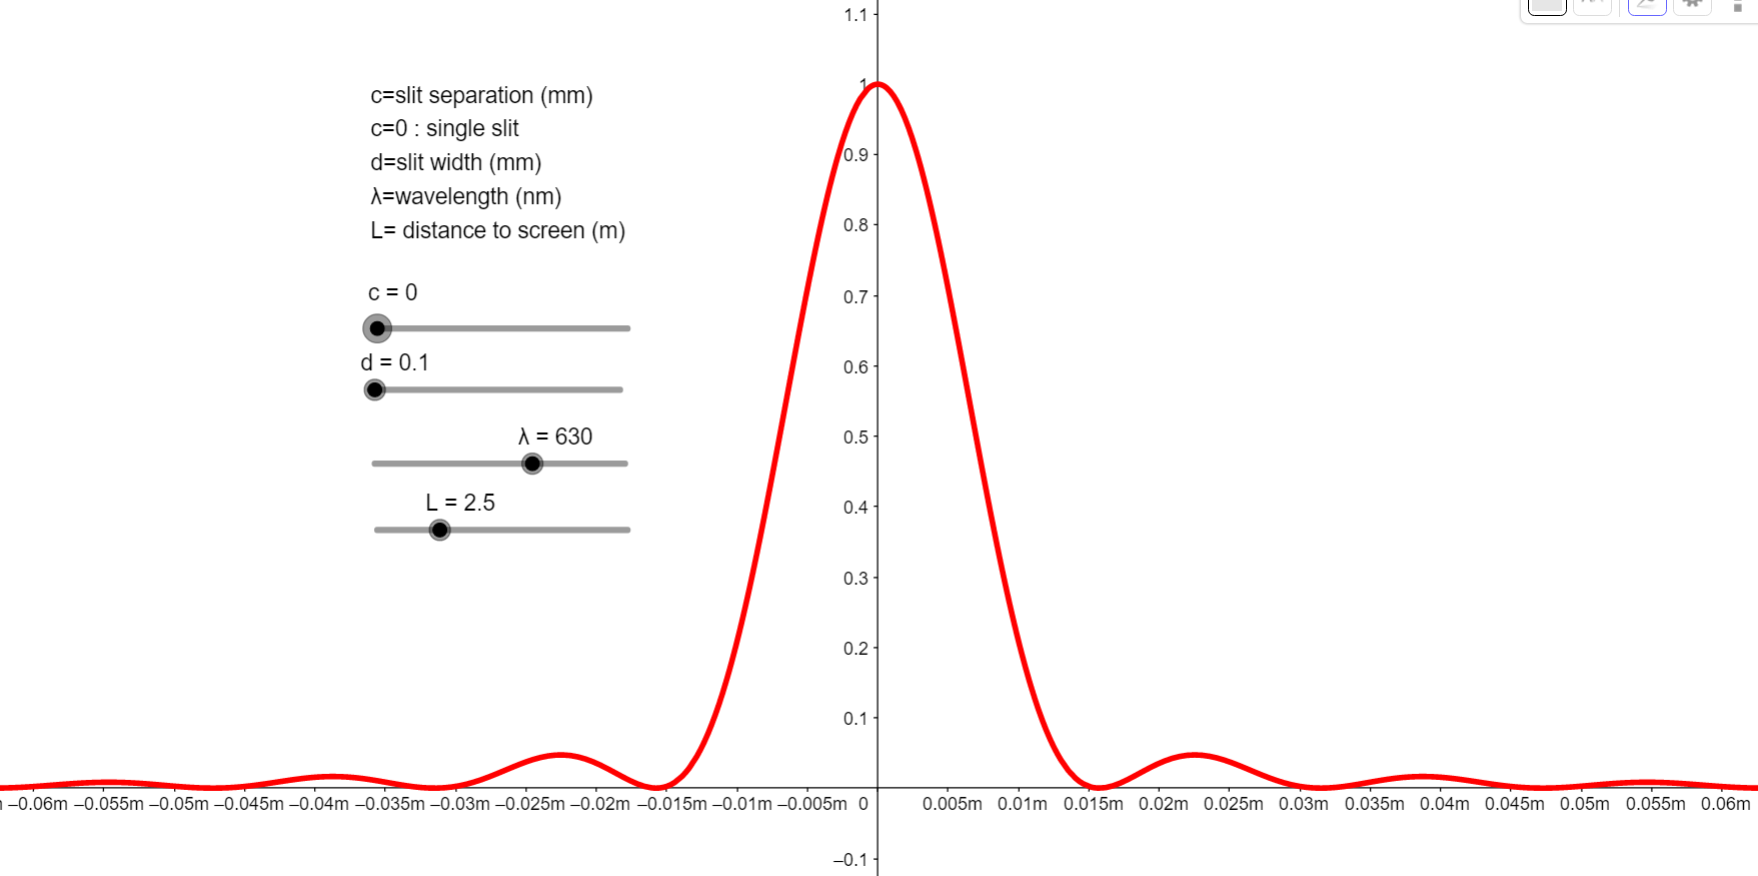
\includegraphics[width=1\textwidth]{./img/singleslit.PNG}
\end{minipage}%
\hfill
\begin{minipage}{.45\textwidth}
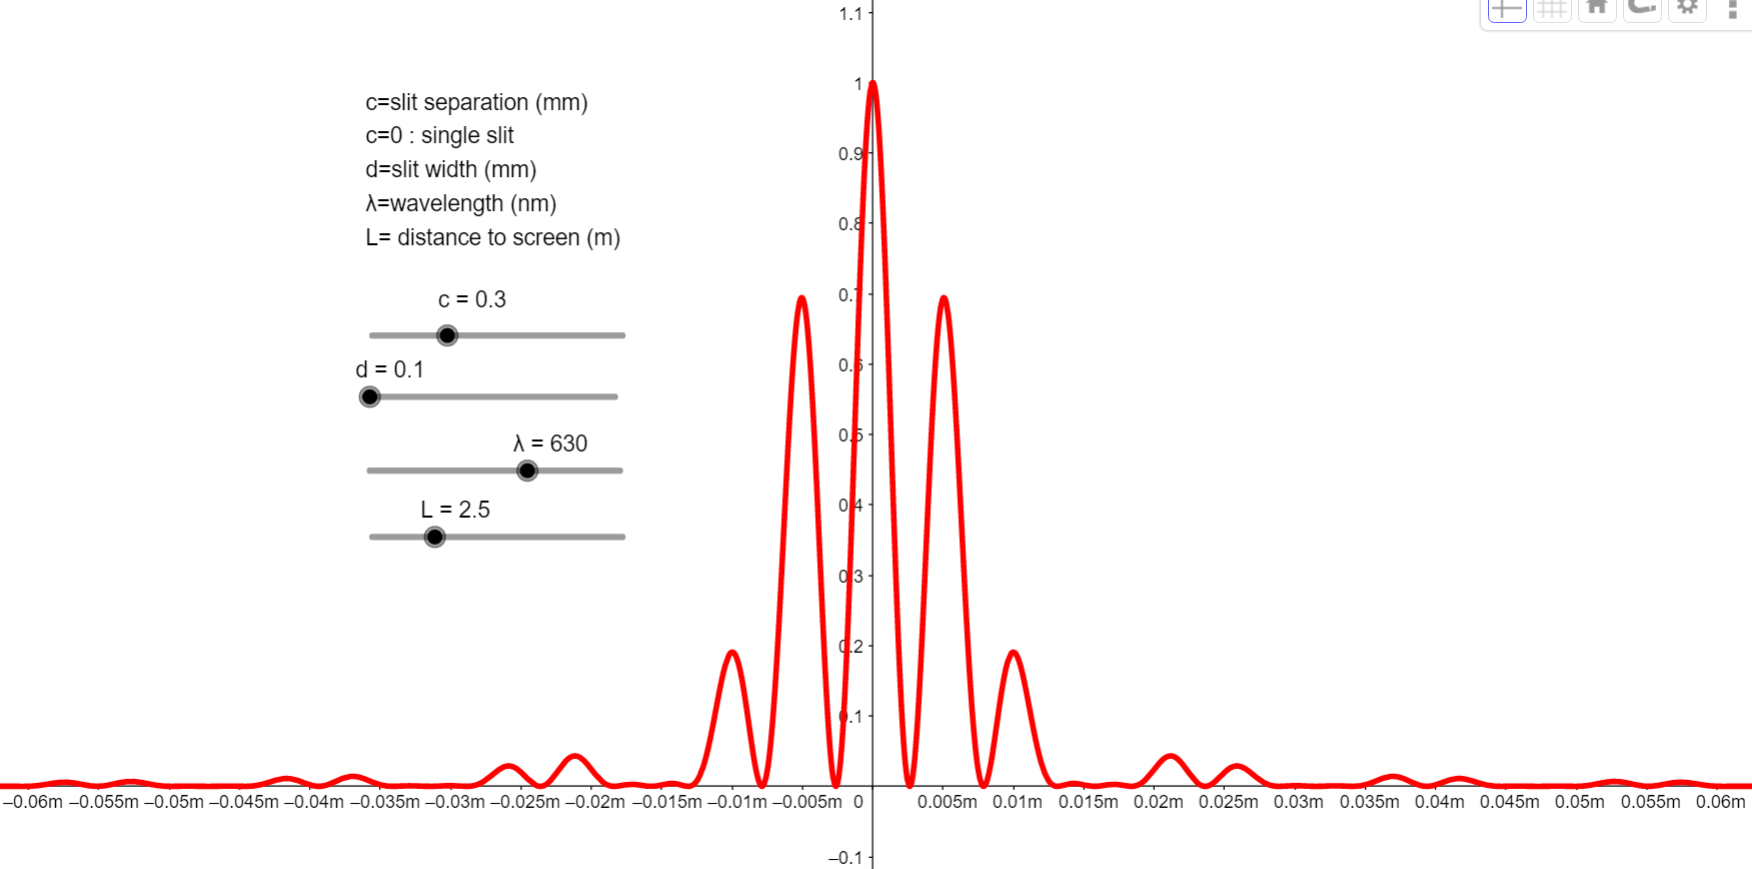
\includegraphics[width=1\textwidth]{./img/doubleslit.PNG}
\end{minipage}
\captionof{figure}{intensiteitspatronen van enkel- (l) en dubbelspleet (r). leg ze op elkaar, benoem de verschillen en de overeenkomsten}
\label{fig:geogebra}
\end{flushleft}


\paragraph*{Les~2:} Polarisatie en wet van Malus.
\begin{itemize}
\item Polarisatie projecteert de amplitude van de $\vec{E}$-component van de lichtvector. De lichtvector is zelf niet waarneembaar. De energie is wel waarneembaar. Het is het kwadraat van de amplitude. Dit is een quantumeigenschap: de amplitude van de lichtvector verhoudt zich tot (kans)amplitude en energie (intensiteit) tot kans.  

\item Het werkblad kan als huiswerk gemaakt worden. Uitgebreide instructie in \cite{monteiro2017polarization} (open access).
Geeft oefening in meten met je telefoon en excelvaardigheid (sjabloon op de site0. Werkblad in dossier.
Nodig: strookje polaroid filter (plm 2x4 cm) en scherm en een smartphone met software.

\item Ik moest \SI{90}{\degree} optellen bij mijn pitchsignaal (draaiing in het verticale vlak) om de ori\"entatie van het filter en mijn scherm in de cosinusverband te laten passen.

\item NB: Sommige schermen (iphones in ieder geval) maken gebruik van circulaire polarisatie. Die kunnen niet als bron gebruikt worden (wel om mee op te nemen natuurlijk). Vandaar de check op het oog vooraf.

\item Het gebruik van absolute en relatieve referentie in Excel is lang niet aan iedere leerling bekend.
Dit experiment geeft inzicht in het begrip van amplitude, kans, som van kansen $sin^2+cos^2=1$, grafische voorstelling, orthogonale componenten.  
\end{itemize}


Je ruwe metingen lijken op die in figuur~\ref{fig:maluslaw}. 
\marginpar{\vspace{-.5cm}
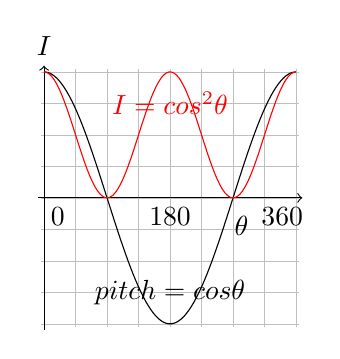
\begin{tikzpicture}[scale=.4,domain=0:8, samples=100]
\draw[very thin,color=lightgray] (-0.1,-4.1) grid (8.1,4.1);
\draw[->] (-0.2,0) -- (8.2,0) node[below, xshift=-22, yshift=-3] {$\theta$};
\draw[->] (0,-4.2) -- (0,4.2) node[above] {$I$};
\draw[color=black] plot (\x,{4*(cos{(\x*45)})});
\node at (4,-3) {$pitch = cos{\theta}$};
\node[below, xshift=5] at (0,0) {${0}$};
\node[below, xshift=0] at (4,0) {$180$};
\node[below, xshift=-5] at (8,0) {$360$};
\node[color=red] at (4, 3) {$I = cos^{2}{\theta}$};
\draw[color=red] plot (\x,{4*(cos{(\x*45)})^2});
\end{tikzpicture}
\captionof{figure}{\footnotesize{Wet van Malus. Onderlinge hoek tussen de filters (zwart), intensiteit van het doorvallende licht (rood).}\label{fig:maluslaw}}
} 
\medskip

\paragraph{Uitvoering}
Doe een paar haarbandjes of een sok om de telefoon zodat de schermen niet krassen. 
Het ligt aan de ori\"entatie van de polarisatie van het scherm en het filter of de cosinuswet er zonder manipulatie uitkomt. Bij mij thuis is de polarisatie van de TV loodrecht op die van mijn laptop. NB polarisatie van smartphones is \SI{45}{\degree} of circulair. Dat is wel zo fijn als je een polaroid bril op hebt.

\marginpar{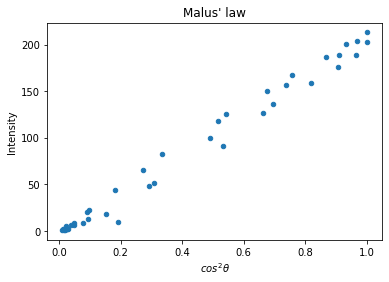
\includegraphics[width=0.95\marginparwidth]{./img/malussmartphone.png}\captionof{figure}{huiswerkopgave. \label {fig:malussmartphone}}}
Fig.~\ref{fig:malussmartphone} geeft een resultaat van het werkblad. Het resultaat had nog geoptimaliseerd kunnen worden door kleine veranderingen in de offset hoek aan te brengen. Bij \SI{92}{\degree} liggen de punten nagenoeg op een lijn. Kennelijk het filter iets scheef geplakt. Hogere excel-kunde: De Excel solver kan deze hoek optimaliseren.


Alternatief als demonstratie

In de klas: als demonstratie en groepsexperiment. De leerlingen hebben allemaal een strookje polaroid.

1. met twee ten opzichte van elkaar draaiende polaroids Een keer rond: Twee keer licht en twee keer donker. Dat lijkt op figuur~\ref{fig:maluslaw}: $cos^2$. 

Teken op het bord: projectie van de \textit{amplitude} van de lichtvector van kruisende filters (projectie van y-as op x-as). 

Bij andere hoeken: Je meet het kwadraat van de amplitude (\textit{intensiteit}, vgl. energie van een trilling evenredig met uitwijking in het kwadraat)

2. Dan een derde filter tussen twee kruisende filters plaatsen. Dit is niet zomaar een grijsfilter. Het wordt lichter. Nogmaals projectie (zie figuur\ref{fig:3pol}).

3. check ook: Indien voor of achter de kruisende filters geplaatst geeft het \SI{45}{\degree} geen effect.

4. Als je het door hebt: N filters onder een hoek $\theta=(90/(N-1))$ met elkaar laten $Ncos^\theta$ licht door. Je kunt het licht zo \SI{90}{\degree} draaien. Hoe meer filters hoe beter de doorlaat. Filters absorberen natuurlijk wel als je de hoek te klein maakt gaat er weer licht verloren... Er is een optimum. 


\textbf{extra opdracht}
De wet van Malus staat het toe om  in principe zonder verlies de polarisatie \SI{90}{\degree} te draaien. Bij kleine $\theta$ gaat $cos^2 \theta$ snel naar 1. Dat betekent bijna \SI{100}{\percent} transmissie. Als je deze truc herhaald kun je een willekeurige hoek draaien. De hele klas heeft een stukje polaroid gekregen. Een samenwerkingsopdracht.
Laat met een fotootje zien dat er nauwelijks absorptie optreedt als het licht door alle filters gaat, en dat er volledige absorptie optreedt als het licht alleen door het eerste en laatste filter gaat. Dat kan in een foto als je het eerste en laatste filter een stukje laat uitsteken. Er is nog een twist: het plastic dragermateriaal absorbeert ook energie. Dat is te onderzoeken door de absorptie te meten van een aantal filters die op elkaar liggen. Het is duidelijk dat bij een al te groot aantal filters er helemaal geen licht meer doorkomt. Is er een optimum aantal filters te vinden waarmee je de polarisatie van het licht \SI{90}{\degree} draait en maximale lichtsterkte doorlaat? 


\paragraph*{Les~3}: Enkel- en dubbelspleet met polarisatie
werkblad~\ref{sec:wbYoung2}.


\textbf{Voorbereiding} het schuifje met de loodrechte films maken. Dat luistert nauw. 
De uitleg van Young2 is lastig, maar de laatste stap is alleen te verklaren met  superpositie. Interferentie!


Quantumprocessen zijn intrinsieke kansprocessen. Het $sinc^2$-patroon bij de enkelspleet en het interferentiepatroon bij de dubbelspleet zijn kansverdelingen. Er is een plek waar het foton het meest waarschijnlijkst komt, en ook plekken waar het nooit mag komen.

\hrefqr[-2cm]{https://www.utwente.nl/en/bms/elan/researchanddevelopment/projects/impuls/deelprojecten/natuurkunde/lesopzetdualiteit.pdf}
{Universiteit Twente} heeft een koffer te leen waarmee het fotonen experiment bij lage intensiteit kan worden uitgevoerd. De link verwijst naar een document met  didactische aanwijzingen voor het gebruik.

\marginnote{\vspace{0cm}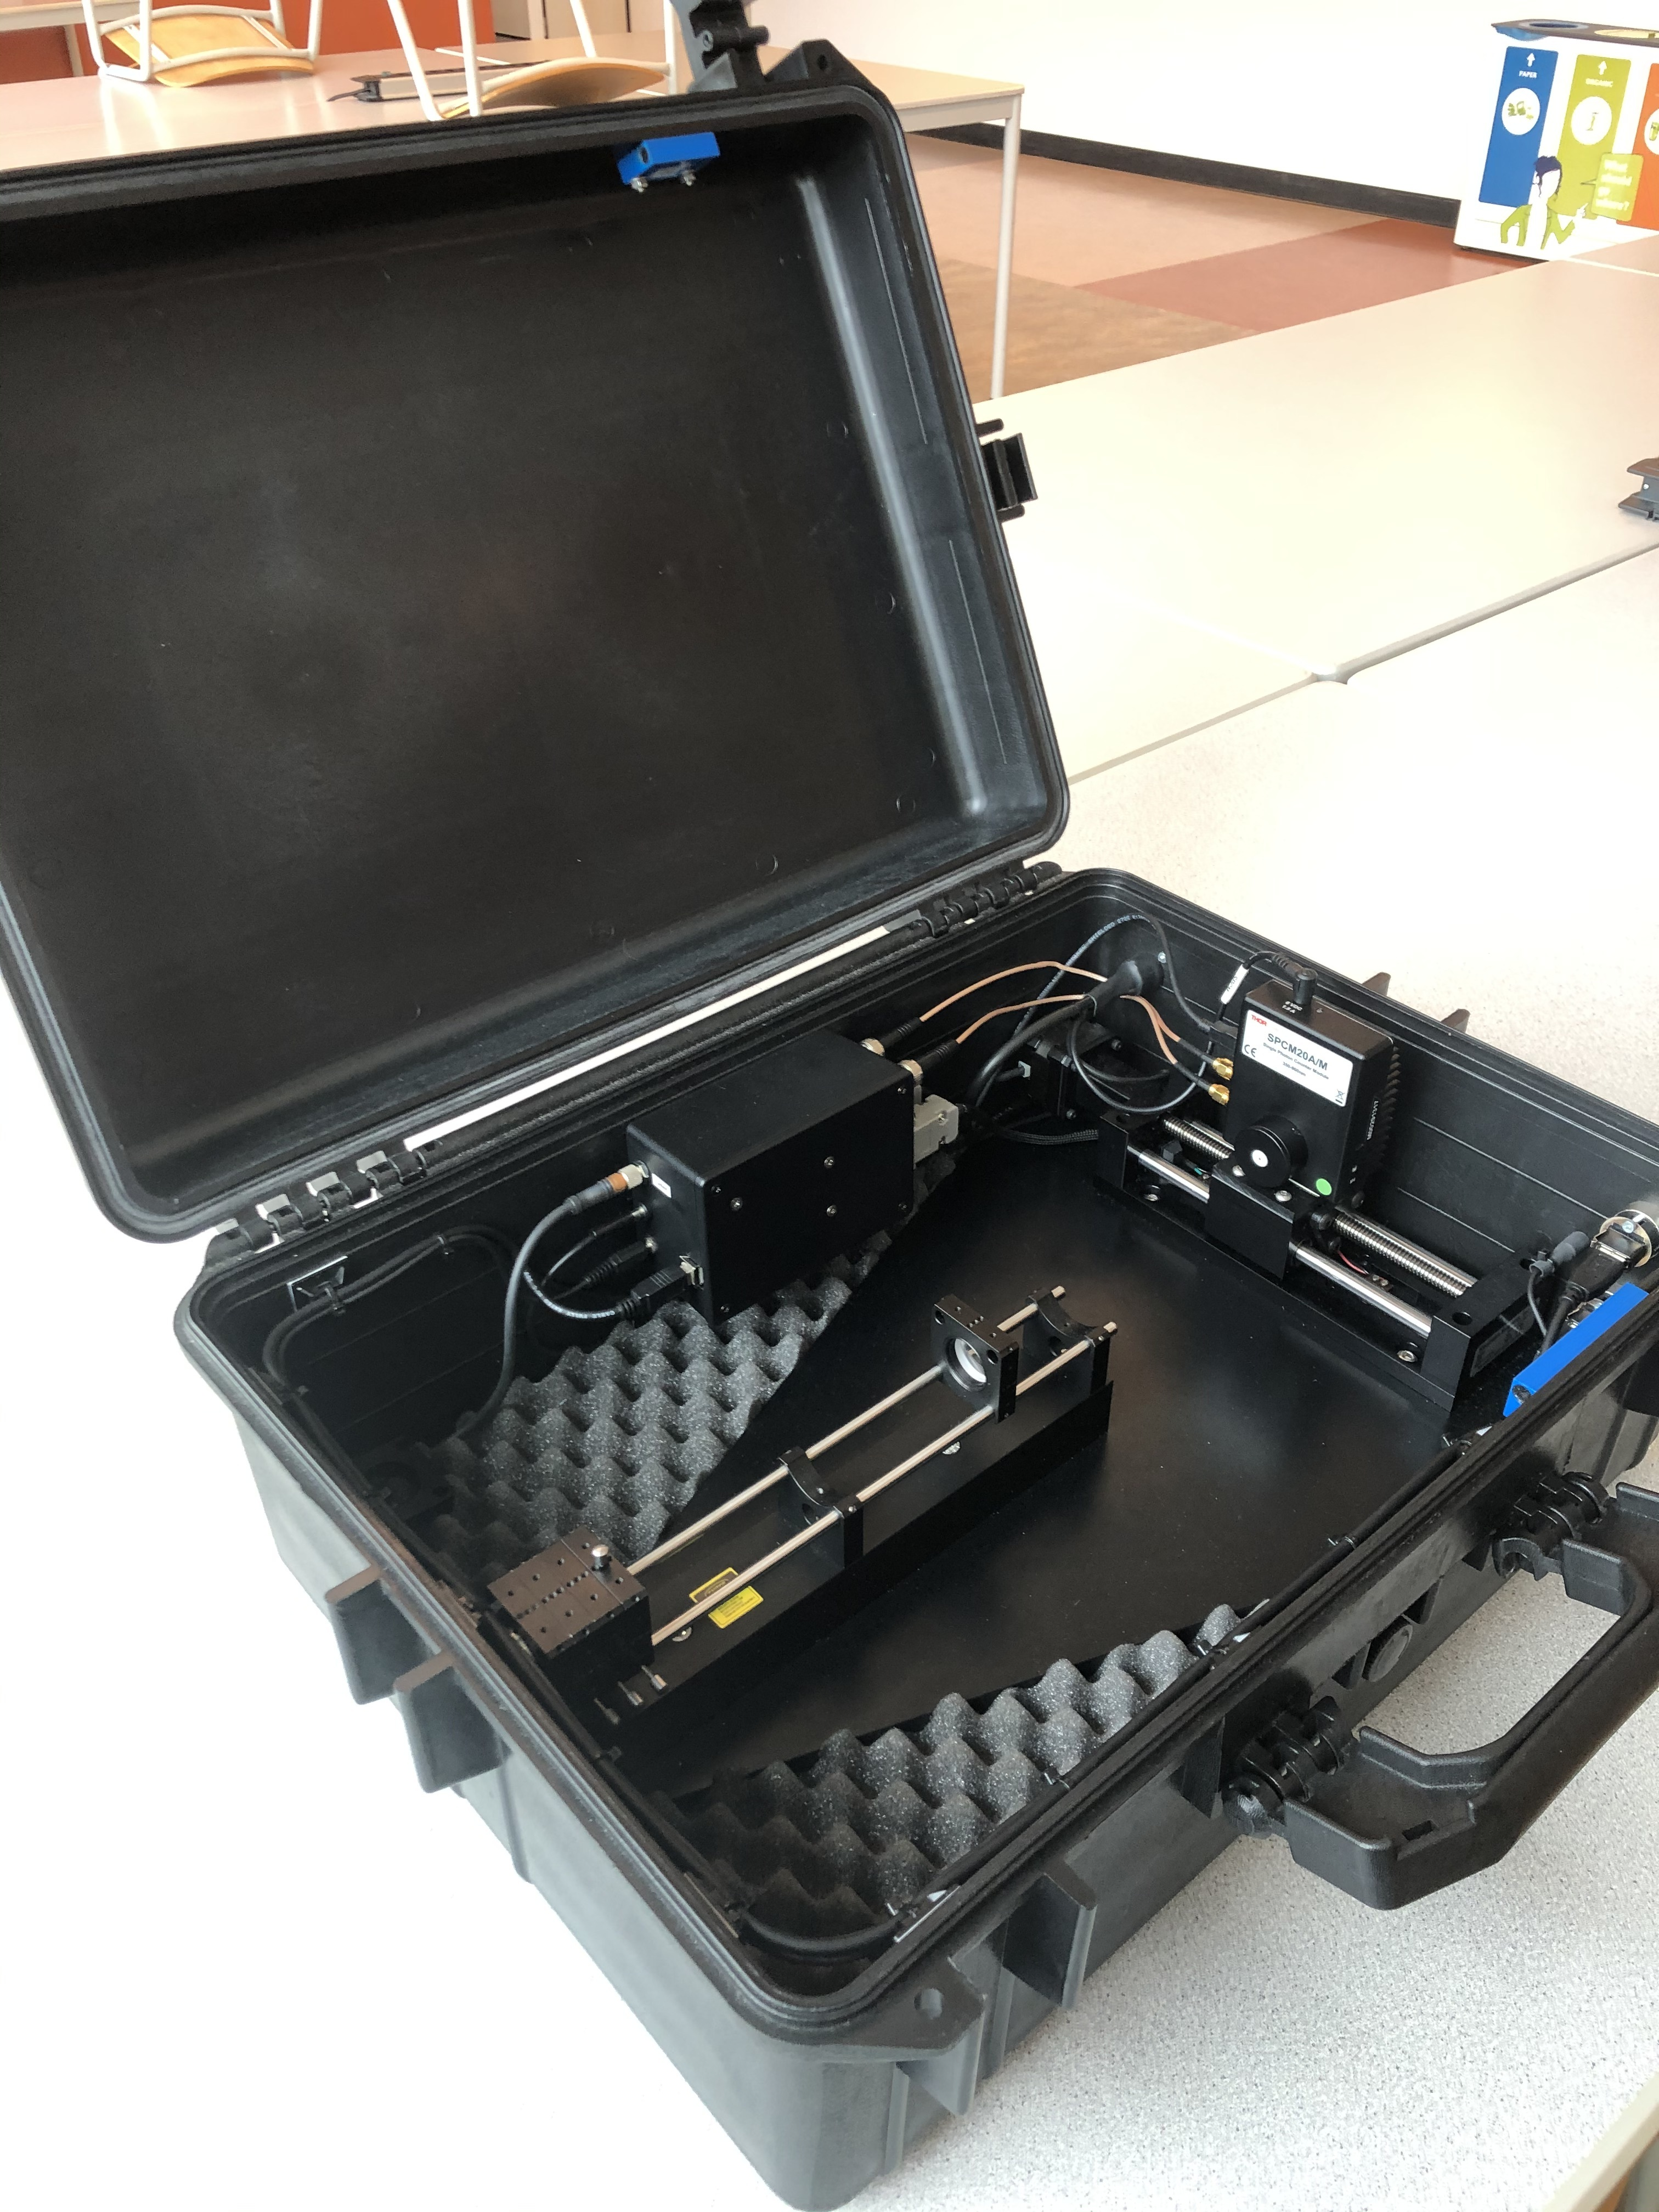
\includegraphics[width=0.95\marginparwidth]{./img/twentekoffer IMG_1138 2.jpeg}\captionof{figure}{te leen in Delft en Enschede. \label {fig:twentekoffer}}}

In een beroemde versie van het \hrefqr[6cm]{https://www.youtube.com/watch?v=1LVkQfCptEs&ab_channel=EmpiricalZeal}{dubbelspleet experiment} (youtube filmpje 1min08, uitgevoerd met elektronen in plaats van fotonen) zie je aanvankelijk op willekeurige plaatsen een puntje verschijnen op het scherm waar een elektron het scherm raakt. Na enige tijd zie je een patroon ontstaan. Het proces is 30~x versneld weergegeven.
 
We hebben kennis gemaakt met kansproces, toestandsvector, lichtvector, amplitude, intensiteit en kans, Interferentie, superpositie, waarneming, een groot aantal metingen levert de kansdichtheid voor een enkele waarneming. Verstrengeling moet nog even wachten.

\subsection*{week 2, H2}
\paragraph*{Les1:} Hoofdstuk 2 begint met een inleiding over klassieke poorten. Dit is  opgenomen om een referentiepunt te bieden ten opzichte van quantumcomputers. Het gaat te ver om hier  diepgaand de werking van klassieke computers aan de orde te stellen. Poorten hebben in het algemeen meer ingangen dan uitgang, bits kun je kopi\"eren met de fan-out.

%Werkblad klassieke computer~\ref{sec:wbklassiek} Een flipflop zelf verzinnen is misschien wat lastig. Internet is je grote vriend. \href{https://www.electronicsforu.com/technology-trends/learn-electronics/flip-flop-rs-jk-t-d}{Hier} staan er een aantal.


\paragraph{Les~2:} Oude vrouw jonge vrouw werkblad~\ref{sec:wbOVJV}.
Kopieer eventueel figuur ~\ref{fig:ovjvFull} in N-voud of zorg dat ieder het kan zien.

Herhalen van de begrippen amplitude en kans en hoe je ze berekent. Verder toestandsvector basis en waarneming met het model Oude vrouw Jonge vrouw (OVJV)

Klassikaal: Uitvoeren van eerste deel van werkblad OVJV~\ref{sec:wbOVJV}. Pen en papier bij de hand. COVID: deel je gegevens in de chat.

Tweede deel is mogelijk huiswerk: bereken je eigen vector. Iemand berekent de verzamelgrafiek van alle waarnemingen van de klas. Bij het bespreken: teken de vector met het klassengemiddelde in.

omrekenen van aantallen waarnemingen naar kans (of percentage)
Terugwerken van kans naar amplitude door de wortel van de kans te nemen. Zowel voor individuele waarneming als voor klassengemiddelde.

Leermomentjes: werken met amplituden en kansen. Superpositie: De tekening  is een superpositie, een waarneming resulteert in \'e\'en van de basistoestanden. Indien vaak herhaald, geeft het experiment aan of de ontwerper goed in zijn poging geslaagd is. Wijs op overeenkomst met natuurkundige experimenten uit H1.

Ga niet te ver met de analogie. 'Een model neemt je eerst bij de hand en later bij de neus.' Wel wijzen op de parallellen van het model met quantum, en even terugkomen op de experimenten van H1:

\begin{itemize}
\item Het is een twee toestandensysteem.
\item Je meet een basistoestand.
\item de tekenaar heeft zijn best gedaan een superpositie te tekenen.
\item Een enkele meting is heeft een random uitkomst, In een echt quantumproces is dit kansproces intrinsiek, in het model is het een onbegrepen neurologisch proces.
\item Als het experiment een groot aantal malen wordt uitgevoerd levert het de kansverdeling in de vorm van een intensiteitspatroon.
\end{itemize}

\paragraph*{Les~3:} Bespreek werkblad OVJV (tweede deel)
Deel de resultaten van de klas. Wie zat het dichtst bij het gemiddelde? Die heeft een zak quantumtum verdiend, wel uitdelen!.
\marginnote{\vspace{-3cm}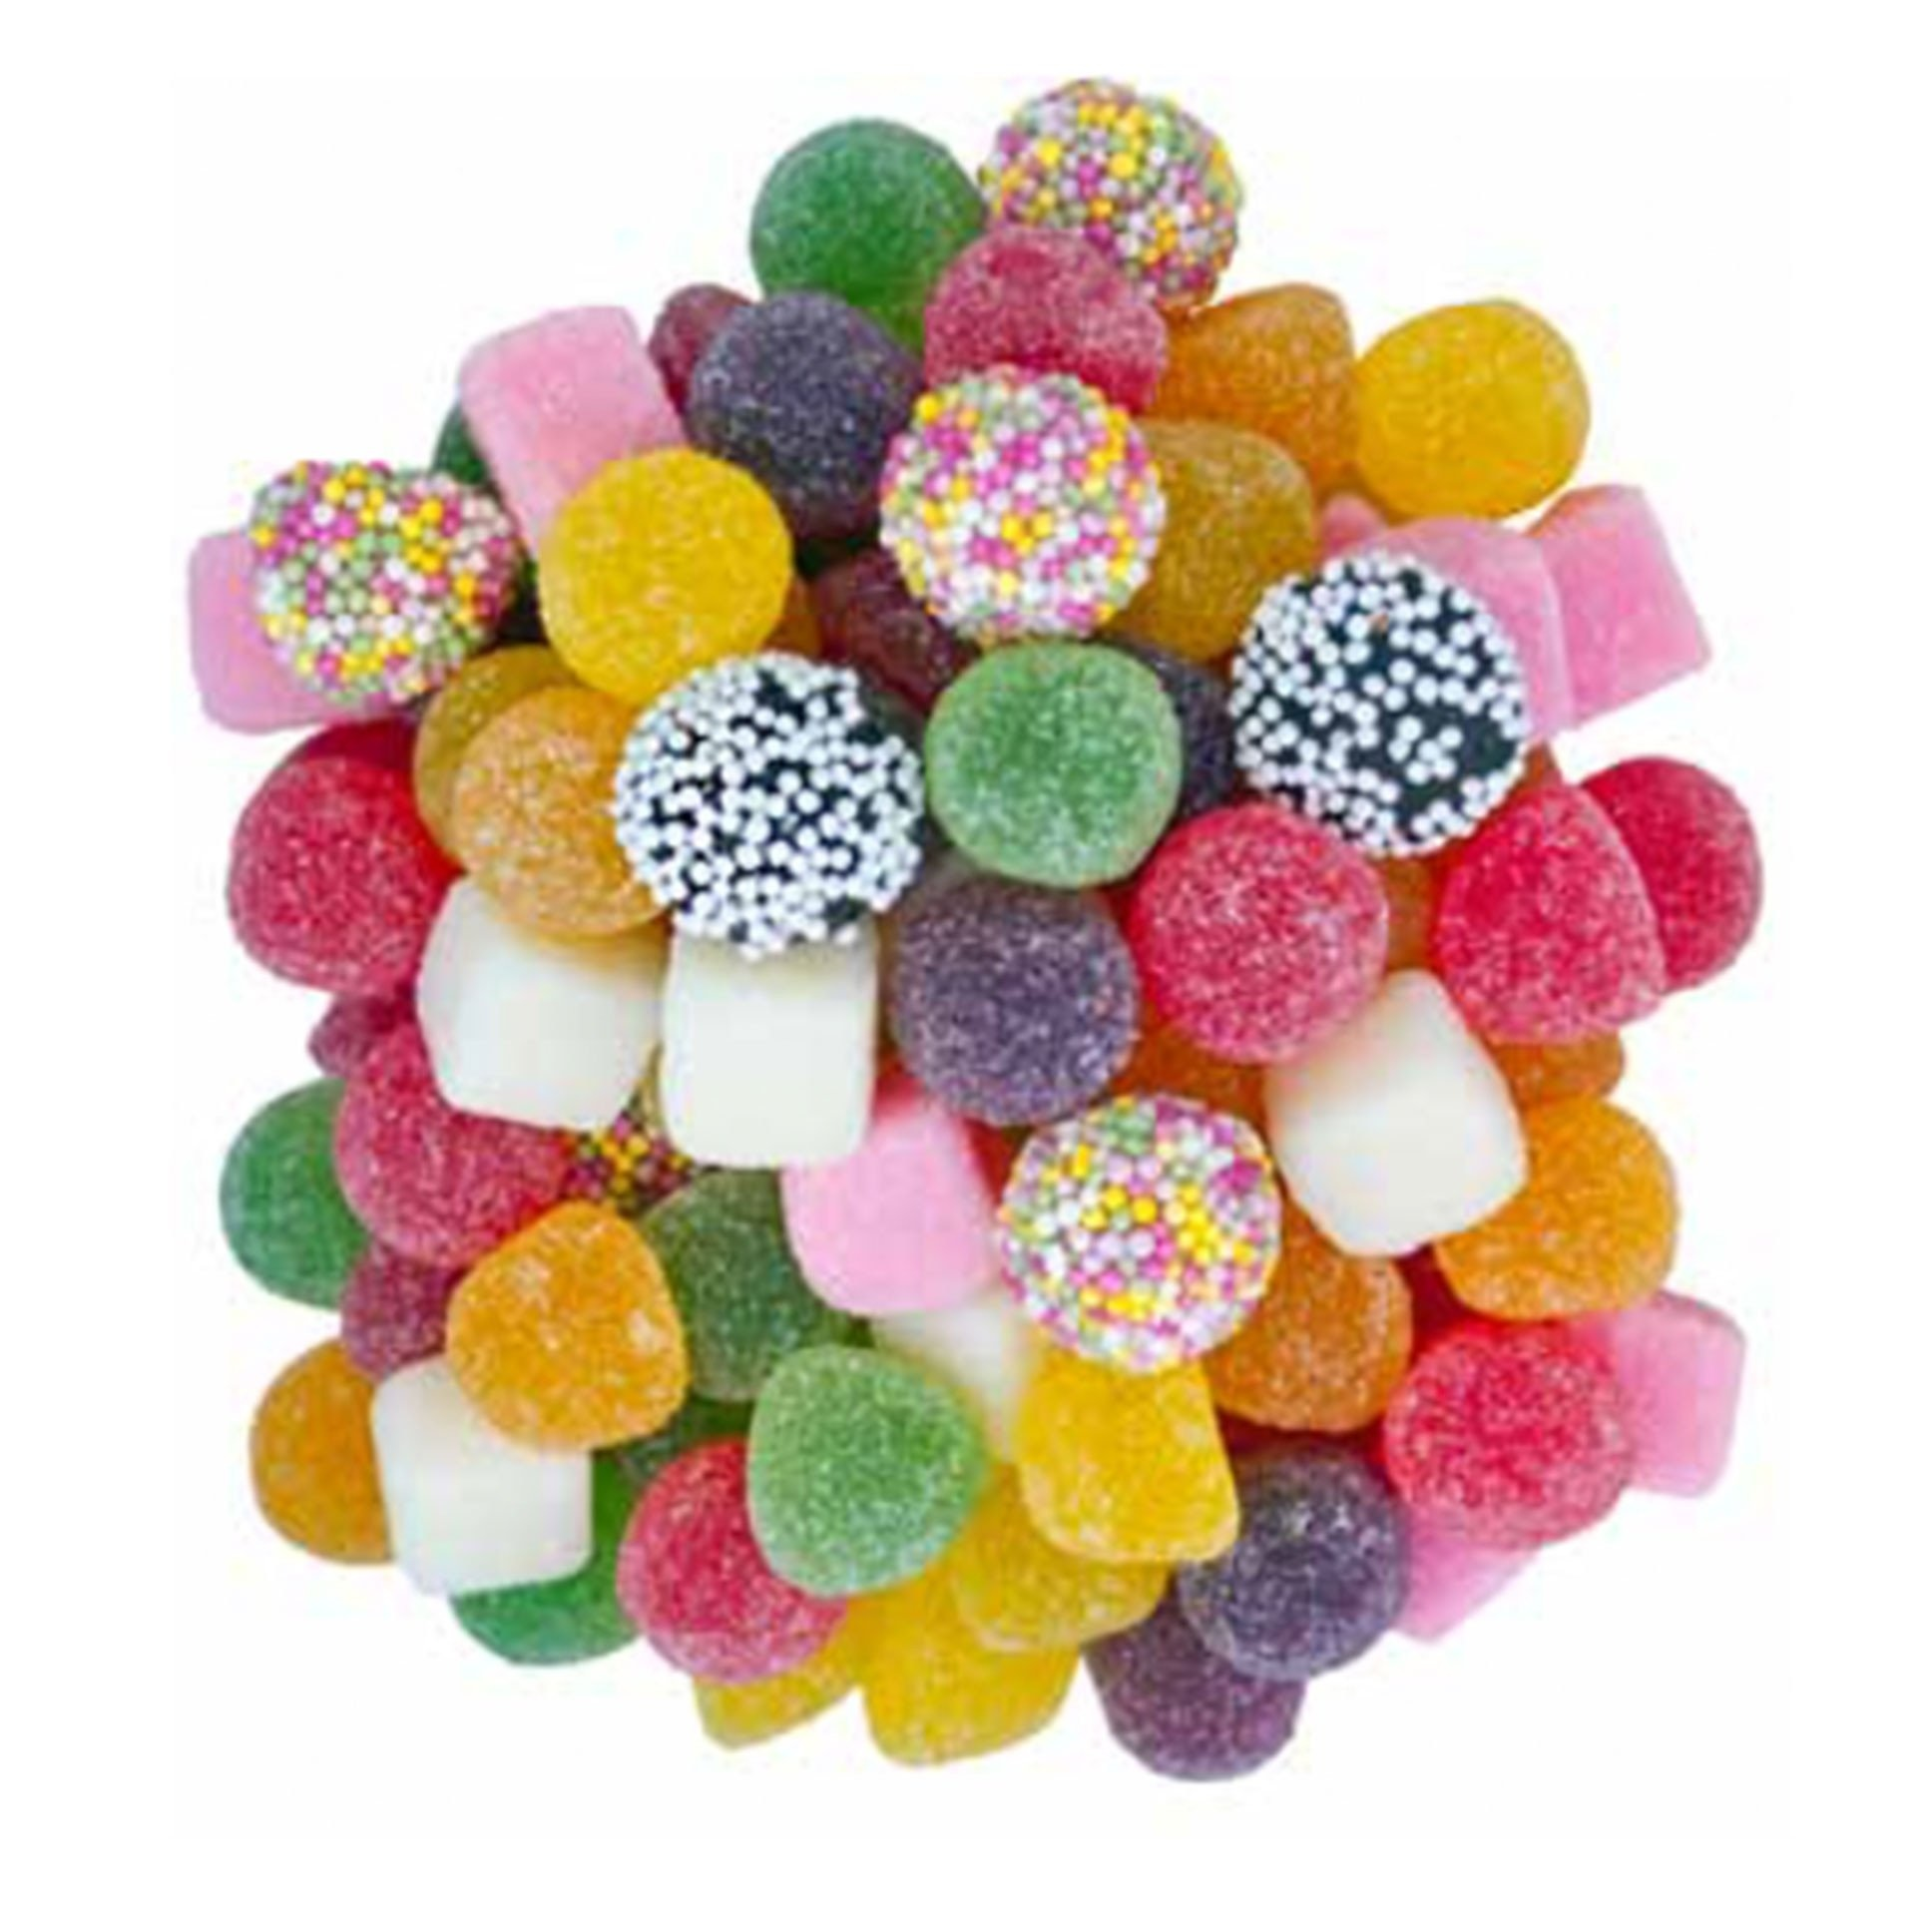
\includegraphics[width=0.95\marginparwidth]{./img/quantumtum.jpg}}

Het meten met verschillende bases~\ref{sec:verschillendebases}

Over het meetprobleem~\ref{sec:meetprobleem}
We volgen de redenering van Runia op opencurve \cite{runiaopencurve}. De helderste uitleg voor ons publiek die we konden vinden 

\textbf{Een Bell-test~\ref{sec:belltest}}
De  afleiding van de Kopenhaagse kansen te doen is te veel schrijfwerk voor de hoofdtekst. Daarom hier in de docentenhandleiding. We schrijven hier het algemene geval ($\alpha$) In de tekst is $\alpha = \tfrac{\pi}{3}$. We moeten eerst de eenheidsvectoren van de verticale basis uitgedrukken in de basis A


\[\ket{0}_V = \cos{\alpha}\ket{0}_A - \sin{\alpha}\ket{1}_A\]
\[\ket{1}_V = \sin{\alpha}\ket{0}_A + \cos{\alpha}\ket{1}_A\]

en voor basis B

\[\ket{0}_V = -\sin{\alpha}\ket{0}_B + \cos{\alpha}\ket{1}_B\]
\[\ket{1}_V = \cos{\alpha}\ket{0}_B + \sin{\alpha}\ket{1}_B\]

We drukken $\Psi= \tfrac{1}{\sqrt{2}}\left(\ket{0}_V\ket{0}_V+\ket{1}_V\ket{1}_V\right)$ uit in basis A
\begin{align*}
\ket{1}_V\ket{1}_V &= \left(\sin{\alpha}\ket{0}_A + \cos{\alpha}\ket{1}_A\right)\left(\sin{\alpha}\ket{0}_A + \cos{\alpha}\ket{1}_A\right) \\
     & = \sin^2{\alpha}\ket{0}_A\ket{0}_A 
       + \cos^2{\alpha}\ket{1}_A\ket{1}_A \\
     & + \sin{\alpha}\cos{\alpha}\ket{0}_A\ket{1}_A
       + \sin{\alpha}\cos{\alpha}\ket{1}_A\ket{0}_A
\end{align*}

\begin{align*}
\ket{0}_V\ket{0}_V &= \left(\cos{\alpha}\ket{0}_A - \sin{\alpha}\ket{1}_A\right)\left(\cos{\alpha}\ket{0}_A - \sin{\alpha}\ket{1}_A\right) \\
     & = \cos^2{\alpha}\ket{0}_A\ket{0}_A 
       + \sin^2{\alpha}\ket{1}_A\ket{1}_A \\
     & - \cos{\alpha}\sin{\alpha}\ket{0}_A\ket{1}_A
       + \cos{\alpha}\sin{\alpha}\ket{1}_A\ket{0}_A
\end{align*}

In $\Psi$ vallen nu de kruistermen weg

\begin{align*}
\Psi & =\tfrac{1}{\sqrt{2}}\left((\sin^2{\alpha}+\cos^2{\alpha})\ket{0}_A\ket{0}_A
       +(\sin^2{\alpha}+\cos^2{\alpha})\ket{1}_A\ket{1}_A\right) \\
     & = \tfrac{1}{\sqrt{2}}\left(\ket{0}_A\ket{0}_A + \ket{1}_A\ket{1}_A\right)
\end{align*}

Dit is de toestand waar we mee vervolgen in de leerlingentekst



\textbf{Kansen volgens EPR}
Wij besloten deze uileg volgens~\cite{bernhardt2019quantum} niet op te nemen in de leerlingenhandleiding, maar we willen deze u ook niet onthouden. Als de gonio uit de leerlingenhandleiding een te grroot obstakel is, kunt u met deze redenering goed het verschil tussen de EPR en Kopenhaagse redeneringen aantonen.

Als we nog eens goed naar figuur~\ref{fig:bellapparaat2} kijken dan zijn er drie bases waarin gemeten kan worden. In elke basis kan de meting er voor zorgen dat een groene of een rode lamp gaat branden. In de klassieke gedachtegang bezit een elektron bij aankomst al een bepaalde spinrichting. Dat geeft een lijst van acht mogelijke uitkomsten. We zouden ons bijvoorbeeld een elektron kunnen voorstellen dat bij meting in de basis V een groene lamp zou laat branden, in de basis A ook een groene lamp en in de basis B weer een groene lamp. We zouden dat elektron kunnen indelen  met het label \textbf{000} (in volgorde \textbf{VAB}). En er zouden elektronen zijn die in alle drie de bases een rode lamp laat branden. Die krijgen het label \textbf{111}.  Er zou ook een label zijn als bijvoorbeeld \textbf{101}. Een elektron uit die groep laat een groene lamp oplichten in basis A maar zal bij de andere bases voor rood licht zorgen.  Er zijn acht van dat soort labels. We kunnen  in de klassieke gedachtegang alle elektronen blijkbaar onderbrengen in acht groepen. Helaas kunnen we een elektron maar \'e\'en keer meten. De meting verstoort zijn richting. Desalniettemin kunnen we bij het experiment van figuur~\ref{fig:bellapparaat2} toch twee keer een meting verrichten. We beschikken immers over elektronparen met gelijke richting.  Alice verricht een meting en Bob een tweede. Er zijn negen verschillende combinaties van de meetbases van Alice en Bob.
Hier zijn die combinaties: V-V, V-A, V-B,  A-V, A-A, A-B, B-V, B-A, B-B. Omdat Alice en Bob hun bases onafhankelijk en volkomen ad-random kiezen kunnen we zeggen dat elke combinatie een kans van 1/9 heeft om gekozen te worden. 
Stel nu: er komt een elektronenpaar  van de groep \textbf{101}. Alice meet in basis B en Bob in basis V. Dat is de zevende combinatie uit de lijst hierboven. In basis B laat elektron \textbf{101} de rode lamp branden en in basis V zorgt dit ook voor een rode lamp. Dat is voor alle mogelijkheden uitgewerkt in tabel~\ref{tab:bellEPR}.

\begin{table}[h]
\begin{tabular}{|>{\columncolor[gray]{0.8}}c|c|c|c|c|c|c|c|c|c|}
\rowcolor{gray}& V-V&V-A&V-B&A-V&A-A&A-B&B-V&B-A&B-B \\ \hline
000 &\textcolor{green}{G}\textcolor{green}{G} &\textcolor{green}{G}\textcolor{green}{G} &\textcolor{green}{G}\textcolor{green}{G} &\textcolor{green}{G}\textcolor{green}{G} &\textcolor{green}{G}\textcolor{green}{G} &\textcolor{green}{G}\textcolor{green}{G} &\textcolor{green}{G}\textcolor{green}{G} &\textcolor{green}{G}\textcolor{green}{G} &\textcolor{green}{G}\textcolor{green}{G}  \\ \hline
001 &\textcolor{green}{G}\textcolor{green}{G} &\textcolor{green}{G}\textcolor{green}{G} &\textcolor{green}{G}\textcolor{green}{R} &\textcolor{green}{G}\textcolor{green}{G} &\textcolor{green}{G}\textcolor{green}{G} &\textcolor{green}{G}\textcolor{red}{R} &\textcolor{red}{R}\textcolor{green}{G} &\textcolor{red}{R}\textcolor{green}{G} &\textcolor{red}{R}\textcolor{red}{R}  \\ \hline
010 &\textcolor{green}{G}\textcolor{green}{G} &\textcolor{green}{G}\textcolor{red}{R} &\textcolor{green}{G}\textcolor{green}{G} &\textcolor{red}{R}\textcolor{green}{G} &\textcolor{red}{R}\textcolor{red}{R} &\textcolor{red}{R}\textcolor{green}{G} &\textcolor{green}{G}\textcolor{green}{G} &\textcolor{red}{R}\textcolor{green}{G} &\textcolor{green}{G}\textcolor{green}{G}  \\ \hline
011 &\textcolor{green}{G}\textcolor{green}{G} &\textcolor{green}{G}\textcolor{red}{R} &\textcolor{green}{G}\textcolor{red}{R} &\textcolor{red}{R}\textcolor{green}{G} &\textcolor{red}{R}\textcolor{red}{R} &\textcolor{red}{R}\textcolor{red}{R} &\textcolor{red}{R}\textcolor{green}{G} &\textcolor{red}{R}\textcolor{red}{R} &\textcolor{red}{R}\textcolor{red}{R}  \\ \hline
100 &\textcolor{red}{R}\textcolor{red}{R} &\textcolor{red}{R}\textcolor{green}{G} &\textcolor{red}{R}\textcolor{green}{G} &\textcolor{green}{G}\textcolor{red}{R} &\textcolor{green}{G}\textcolor{green}{G} &\textcolor{green}{G}\textcolor{green}{G} &\textcolor{green}{G}\textcolor{red}{R} &\textcolor{green}{G}\textcolor{green}{G} &\textcolor{green}{G}\textcolor{green}{G}  \\ \hline
101 &\textcolor{red}{R}\textcolor{red}{R} &\textcolor{red}{R}\textcolor{green}{G} &\textcolor{red}{R}\textcolor{red}{R} &\textcolor{green}{G}\textcolor{red}{R} &\textcolor{green}{G}\textcolor{green}{G} &\textcolor{green}{G}\textcolor{red}{R} &\textcolor{red}{R}\textcolor{red}{R} &\textcolor{red}{R}\textcolor{green}{G} &\textcolor{red}{R}\textcolor{red}{R}  \\ \hline
110 &\textcolor{red}{R}\textcolor{red}{R} &\textcolor{red}{R}\textcolor{red}{R} &\textcolor{red}{R}\textcolor{green}{G} &\textcolor{red}{R}\textcolor{red}{R} &\textcolor{red}{R}\textcolor{red}{R} &\textcolor{red}{R}\textcolor{green}{G} &\textcolor{green}{G}\textcolor{red}{R} &\textcolor{green}{G}\textcolor{red}{R} &\textcolor{green}{G}\textcolor{green}{G}  \\ \hline
111 &\textcolor{red}{R}\textcolor{red}{R} &\textcolor{red}{R}\textcolor{red}{R} &\textcolor{red}{R}\textcolor{red}{R} &\textcolor{red}{R}\textcolor{red}{R} &\textcolor{red}{R}\textcolor{red}{R} &\textcolor{red}{R}\textcolor{red}{R} &\textcolor{red}{R}\textcolor{red}{R} &\textcolor{red}{R}\textcolor{red}{R} &\textcolor{red}{R}\textcolor{red}{R}  \\ \hline
\end{tabular}
\end{table}
\captionof{table}{Kolommen: Baiskeuze van resp. Alice en Bob. Rijen: Alle mogelijke uitkomsten van metingen voor de drie bases (VAB). De cellen geven de uitkomsten voor de combinaties basiskeuze en eigenschap (label) van het elektron \label{tab:bellEPR}}

De kolommen leveren allemaal gelijke waarschijnlijkheid voor rood en groen. In de rijen is dat niet het gevel. Er kunnen meer elektronen zijn met het ene label dan het andere label. Maar het valt op dat er bij elk label minstens vijf van de negen kolommen dezelfde kleur hebben. Dat betekent dat de kans op gelijke kleur voor elk label minstens $\tfrac{5}{9}$ moet zijn. De Kopenhaagse opvatting voorspelt daarentegen een kans van precies $\tfrac{1}{2}$ voor een meting met gelijke kleur. 


\textbf{Divincenzo criteria~\ref{sec:divincenzo}}
De cirteria lijken vanzelfsprekend, maar zijn wel de hindernissen die genomen moeten worden bij het bouwen van een quantumcomputer. Het vierde criterium komt in Hoofdstuk~3 pas aan de orde, hier slechts een blik vooruit.

Het bewijs van het no-cloning principe wordt in opdracht~\ref{opd:nocloning}  behandeld.


\subsection*{week3, H3}

\paragraph*{Les~1}
rekenregels. lineariteit is intu\"itief. De 'Brexit'-opdracht ~\ref{opd:lineair} laat dat zien. 

Uitwerken van tensorproduct is gewoon 'papegaaienbekken':
\[(a+b)(c+d)=ad+ad+bc+bd\]

De werking van de \port{I}, \port{X} en \port{Z}-poort moet lukken. De \port{H}-poort is lastiger. Het toestandsdiagram maakt het makkelijk.

Figuur~\ref{fig:PWstateXZH} is een cheatsheet met het toestandsdiagram voor de \port{X}-, \port{Z}- en \port{H}- poort. Die mag je er vast bijhouden tijdens het proefwerk.

Er is geen werkblad bij dit gedeelte

\paragraph*{Les~2} Werkblad Quantum Inspire (Delft)~\ref{sec:wbQI}.
Check vooraf of de webinterface is vernieuwd.

\paragraph*{kopofmunt}\label{sec:kopofmunt}~\ref{opd:kopofmunt}
Deze opdracht illustreert de werking van XHZ poorten in \'e\'en register. \textbf{De instructie moet alleen aan de spelleider bekend zijn}

Speel dit spel met twee spelers en een spelleider. \textbf{LET OP! Zorg dat slechts de spelleider de tekst leest en uitleg geeft aan de spelers}.

Ken je die situatie; dat je iets moet beslissen, maar er niet uitkomt. Bijvoorbeeld als je met een vriend hebt afgesproken en hij wil graag naar de bioscoop, terwijl jij liever wilt gaan basketballen. In zo'n situatie kun je een muntje opgooien, dat is wel zo eerlijk. In dit spel spelen we een variatie op kop en munt met speler~A, Alice en speler~B, Bob.

\paragraph*{Deel 1}
Een ronde van dit spel werkt als volgt. De spelleider legt een muntje op tafel. Het muntje begint altijd in kop. De spelers kunnen twee dingen doen: ofwel het muntje draaien (van kop naar munt, of van munt naar kop), ofwel niks doen (munt blijft munt en kop blijft kop). Eerst geeft Alice haar keuze in het geheim aan de spelleider door (draaien of niks doen), vervolgens doet Bob dit en tot slot mag Alice nog een keer haar keuze doorgeven. In totaal worden er dus per ronde drie operaties (telkens draaien of niets doen) op het muntje uitgevoerd. De spelleider onthoudt steeds de toestand van het muntje (kop/munt) en onthult uiteindelijk de eindstand van het muntje. Als het muntje eindigt in kop, dan wint Alice, eindigt het muntje als munt, dan wint Bob.
\begin{enumerate}
\item Wat is de kans dat Alice wint en wat is de kans dat Bob wint?
\item Als je acht rondes speelt, hoe vaak verwacht je dan dat Bob wint?
\item Wat is de kans dat, na vijf rondes, Bob alle rondes heeft gewonnen?
\item Speel vijf rondes. Komt dit (ongeveer) overeen met jullie verwachtingen?
\item Kun je makkelijk valsspelen?
\end{enumerate}

\paragraph*{Deel 2}
We gaan het spelletje 'iets' veranderen. In plaats van kop, of munt, spelen we het spelletje nu met een qubit. De spelleider prepareert een qubit in de toestand $\ket{0}$ - dit kan op papier. Nu mag eerst Alice het qubit roteren; ze mag kiezen uit niets doen, of een \port{X}-poort ($\ket{0}$ wordt $\ket{1}$ en $\ket{1}$ wordt $\ket{0}$), een flip. Daarna mag Bob het qubit roteren (niets doen, of een flip) en tot slot mag Alice het qubit nog een keer roteren (niets doen, of een flip). Tot slot 'meet' de spelleider het qubit. Als het qubit eindigt in de toestand $\ket{0}$ dan wint Alice, eindigt het qubit in $\ket{1}$ dan wint Bob.

\begin{enumerate}
\item Het qubit begint in $\ket{0}$. Als Alice niets doet, Bob een \port{X}-poort uitvoert en Alice ook een \port{X}-poort uitvoert, in welke toestand eindigt het qubit dan?
\item Wat is de kans dat Bob de ronde wint? (maak eventueel een boomdiagram met alle mogelijkheden)
\item Speel vijf rondes van het spel. Hoe vaak won Alice, hoe vaak won Bob?
\end{enumerate}

\paragraph*{Deel 3}
Alice heeft intussen door dat ze met een qubit te maken heeft en bedenkt wat slims. In plaats van een X-rotatie, besluit ze een Hadamard-poort toe te passen tijdens haar beide beurten. \textit{Aan de spelleider: geef dit - in het geheim - door aan Alice}. 
Bedenk dat een Hadamard poort de toestand $\ket{0}$ verandert in $\ket{+}$ en de toestand $\ket{1}$ verandert in $\ket{-}$.
\begin{enumerate}
\item Speel nu acht rondes van het spel. Hoe vaak heeft Alice gewonnen?
\item Aan Bob: vind je het logisch dat Alice telkens wint? Hoe denk je dat ze dat heeft gedaan?
\item Is er een mogelijkheid dat Bob op deze manier het spel kan winnen?
\end{enumerate}

\paragraph{Les~3}
\port{H}-poort voorbeeld: Ga na dat de toestand genormeerd is. $\alpha^2+\beta^2=1$

\textbf{Meerdere poorten achter elkaar:} Je mag ook $(\port{Z}\port{H})\ket{\Psi}$
 uitrekenen. Associatief, maar niet commutatief, dus niet $\port{H}\port{Z}\ket{\Psi}$.
 
Teken het toestandsdiagram waarmee een \port{$R_y45$} $\ket{0}$ uiteindelijk op zichzelf afbeeld. Hint uit hoeveel elementen bestaat je diagram?
  
Er is ruimte voor meer rekenvragen. Wat doet een $(\port{X}\port{Z}\port{H})$ operatie met de toestand $\ket{1}$. Wat is de andere co\"effici\"ent van de toestand $\alpha=\tfrac{1}{3}$.


Opgave verstrengeling ~\ref{opd:verstrengeling} is belangrijk.

Vraag: teken de actie van de \port{I}-poort in het toestandsdiagram. Geef aan met letter I.

Vraag: Voor welke toestanden werkt de \port{Z}/\port{X}/\port{H} poort als de identiteit?

\paragraph*{werkblad teleportatie}

\begin{enumerate}[wide, labelwidth=!, labelindent=0pt]
\item c
\item b
\item Nee, Je meet een toestand $\ket{0}$ met een kans $\alpha^2$ of $\ket{1}$ met kans $\beta^2$.
\item Je kunt de toestand telkens opnieuw bouwen en het kansproces herhalen. Zo kun je uiteindelijk de co\"effici\"enten benaderen. die gelden tot het qubit gemeten wordt.

\item I, f)X, g)Z, h)XZ


%\item $\ket{11}$ \implies $\alpha\ket{1}-\beta\ket{0}$
%\item 
\item Bob's qubit is instantaan vastgelegd als Alice meet, echter ze moet Bob eerst opbellen (klassiek kanaal) om haar resultaat door te geven. Dat gaat niet sneller dan het licht.
\item Een lamp is geen quantumobject,  laat staan dat een persoon dat is.  Vraag is natuurlijk of het theoretisch verboden is, dat niet.
\item Dat gaat ook maar met een andere decodering, Bob moet andere operaties toepassen, dusus wel afspraken maken vooraf.
\end{enumerate}



\iffalse%eruit--==--==--==


\paragraph*{les 2}Registers
\nogdoen{aanwijzingen hier}
\paragraph*{les 3} Verstrengeling.
\nogdoen{aanwijzingen hier}

\paragraph*{no-cloning}\label{sec:nocloning}
\nogdoen{is nu opgenomen in de leerlingen tekst}

Het is niet mogelijk om een qubit te kopi\"eren, dit is fysisch verboden. In de natuurkunde wordt dit ook wel het 'no cloning theorem' genoemd. Het is best onhandig dat we niet zomaar qubits kunnen kopi\"eren, want dat betekent dat we niet zo makkelijk qubit toestanden kunnen namaken, iets wat we wel graag zouden willen om bijvoorbeeld fouten in een quantumberekening op te sporen (als je drie keer precies dezelfde berekening doet, heb je meer kans dat je op het goede antwoord uitkomt).


Om te kopi\"eren hebben we een qubit nodig die als mal dient. We nemen daarvoor  $\ket{0}$:

\begin{align}\label{eq:copy}
\port{U}\ket{\Psi}\ket{0}=\ket{\Psi}\ket{\Psi}
\end{align}

Stel dat er een poort bestaat die een bit kan kopi\"eren. 
\[ \port{U}\ket{00} = \ket{00} en \port{U}\ket{10}=\ket{11}\]

De afzonderlijke operaties mogen we samenvoegen (in superpositie brengen). We passen daarbij de regels van lineariteit toe (\nogdoen{ref}):

\[\begin{aligned}
\port{U}\left(\tfrac{1}{\sqrt{2}}\left(\ket{00}+\ket{10}\right)\right)=\tfrac{1}{\sqrt{2}}\left(\port{U}\ket{00}+\port{U}\ket{10}\right)=
\tfrac{1}{\sqrt{2}}\left(\ket{00}+\ket{11}\right)
\end{aligned}\]


Je kan de toestand $\ket{0}$ buiten haakjes halen
\[\begin{aligned}
\tfrac{1}{\sqrt{2}}\left(\ket{00}+\ket{10}\right)=
\tfrac{1}{\sqrt{2}}\left(\ket{0}+\ket{1}\right)\ket{0}=
\frac{\ket{0}+\ket{1}}{\sqrt{2}}\ket{0}
\end{aligned}\]


\[\begin{aligned}
\port{U}\bigg(\frac{\ket{00}+\ket{10}}{\sqrt{2}}\bigg)&=\nonumber\\
\port{U}\bigg(\frac{\ket{0}+\ket{1}}{\sqrt{2}}\ket{0}\bigg)&\stackrel{\text{pas vgl.~\ref{eq:copy} toe}}{=}\nonumber
\bigg(\frac{\ket{0}+\ket{1}}{\sqrt{2}}\bigg)\bigg(\frac{\ket{0}+\ket{1}}{\sqrt{2}}\bigg)&=\nonumber\\
\frac{1}{2}(\ket{00}+\ket{01}+\ket{10}+\ket{11})&\neq \nonumber
\frac{1}{\sqrt{2}}((\ket{00}+\ket{11})&\nonumber
\end{aligned}\]

NB. De mal voor het te kopi\"eren qubit kan ook $\ket{1}$ zijn (vgl.~\ref{eq:copy}).
Hoe zit het als $\ket{\Psi}$ met $\ket{0}$ en $\ket{1}$
\fi
\iffalse%-t-t-t-t
\nogdoen{losse opmerkingen moet en eruit:}
Quantumsoftware: in tegenstelling tot klassiek zijn er niet zo veel quantumalgoritmen. Voor een overzicht \cite{Jordan2021} 

De uitleg in de paragraaf over Shor volgt de uitleg van \hrefqr{https://www.youtube.com/watch?v=lvTqbM5Dq4Q&ab_channel=minutephysics}{minutephysics}. Het filmpje zelf is een didactische ramp. Het is alleen begrijpelijk voor degenen die het al begrijpen. 

Shor: enige referenties: bachelor scriptie Sanne Veenstra \cite{Veenstra2018} legt RSA uit (getaltheorie \'en geeft aan hoe Shor's algoritme het vinden van sleutels versnelt. 

Een mooi werkboekje van de Vlaamse wiskunde docent Luc van den Broeck beperkt zicht tot RSA, maar doet dat stap voor stap aan de hand van opdrachten op het niveau van wisD. Ik kon het alleen vinden op docplayer, een dubieuze site \cite{Broeck2017}. Inmiddels contact met de auteur hij heeft me de meest recente versie toegestuurd. (geen antwoorden).

Een prachtig profielwerkstuk over het onderwerp: \cite{Tess2020}


In een \hrefqr{https://www.youtube.com/watch?v=6qD9XElTpCE&ab_channel=Qiskit}{lezing} (30 min) legt Peter Shor geeft de geschieden van zijn ontdekking uit. Hij staat daarbij stil bij het breken van quantum met local realism, gaat uitgebreid in op de ontwikkeling van het algoritme en bespreekt het probleem (en zijn oplossing) van error correction, dat wij in de module niet behandelen.

verschil tussen exponentieel en polynomisch moet lukken


venndiagram oefenen

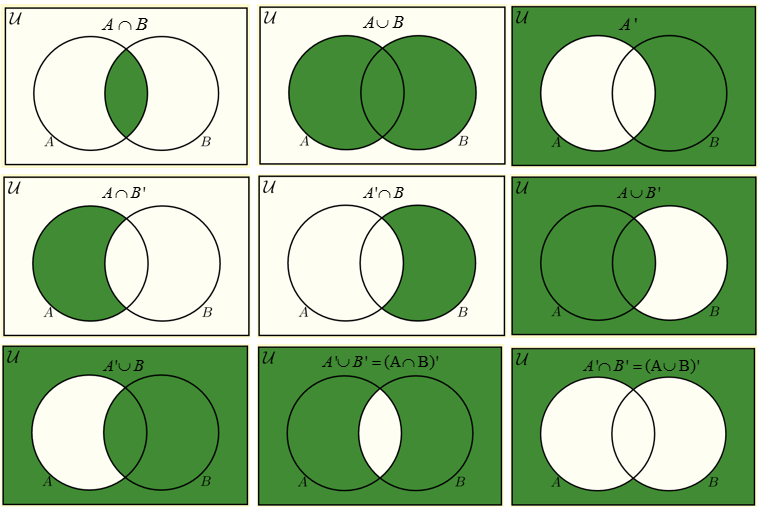
\includegraphics[width=\textwidth]{./img/venn-diagrams.png
}\captionof{figure}{oefenen met venndoagrams. \label{fig:venn}}
\fi%-t-t-t-t

\section{uitwerking opdrachten}
(werkbladen staan apart uitgwerkt in paragraaf~\ref{sec:uitwerkbladen})

\subsection*{hoofdstuk 1}

\textbf{Opzoekvraag in de tekst:}~\cite{timeline2021}
Ik kom op 1988, een NMR systeem

\textbf{exp 1.2 Young1} werkblad~\ref{sec:wbYoung1}

\textbf{exp 1.3 Malus} werkblad~\ref{sec:wbmalus}

\textbf{exp 1.4 Young2} werkblad~\ref{sec:wbYoung2}

\textbf{Opdr 1.5 Enkel foton experiment}~\ref{opd:enkelfotonexp}

Terzijde: de benaming van neutral density filters kent nogal wat variaties. \hrefqr[0cm]{https://en.wikipedia.org/wiki/Neutral-density_filter\#Ratings/}{Hier} een overzicht.

E\'en foton onderweg over een afstand van \SI{30}{\centi\meter} met $c=\SI{3e8}{\meter\per\second}$ komt dat overeen met een verblijftijd  van \SI{1}{\nano\second}.
De bundel zendt \SI{1}{\milli\watt} uit. Energie per foton: $E=\tfrac{hc}{\lambda}$
met $h=\SI{6.62E-34}{\joule\second}$, $\lambda=\SI{635E-9}{\meter}$
levert

$E_f=\tfrac{hc}{\lambda} \implies \SI{3.1E-19}{\joule\per foton}$
gewenst vermogen: $P=E/t=\tfrac{\SI{3.1E-19}{\joule\per foton}}{\SI{1E-9}{\second\per foton}}=\SI{3.1E-10}{\joule\per\second}$

Verzwakking: $\tfrac{1E-3}{3.1E-10}=\num{3.2E6}$. Dit is een ondergrens. Je moet \num{1e7} keer verzwakken, twee ND2 en \'e\'en NG3 filter dus.

\subsection*{Hoofdstuk 2}

\textbf{exp 2.1 klassiek} werkblad~\ref{sec:wbklassiek}
\textbf{exp 2.1 OVJV1}werkblad~\ref{sec:wbOVJV}


\textbf{Opdr}~\ref{opd:inzoomen} Inzoomen
Je moet afdalen tot de \textit{nanowereld} Een factor $\num{1E9}$ dus.
Een atoom is ongeveer een \SI{1}{\angstrom} groot. Het plaatje een decimeter. Dan kom je er ook op uit. 

\textbf{exp 2.1 OVJV1}werkblad~\ref{sec:wbOVJV}

\textbf{opdr}~\ref{opd:herhaal}

Het filter staat verticaal, meet toestand $\ket{1}$.

$\beta^2=\tfrac{3}{4} \implies$\\ $\beta=\pm\tfrac{1}{2}\sqrt{3}$

$\alpha^2+\beta^2=1 \implies$\\ $\alpha=\pm\tfrac{1}{2}$

Hoek met verticaal= \SI{30}{\degree} NB er zijn vier mogelijkheden,
$\pm \SI{30}{\degree}$ en $\pm \SI{150}{\degree}$ t.o.v. $y-as$.

%---

\textbf{Opdr}~\ref{opd:basiscoef} 
\begin{flushleft}
\begin{minipage}{.75\textwidth}
\def\gcolor{green!60!black}
\def\ojfrangle{0}
\def\ojobangle{45}
\def\statangle{-15}%kennelijk relatief aan groene basis
\def\ojscale{.65}
\begin{tikzpicture}%
\clip (-1.7,-4) rectangle (4,4);
\begin{scope}[scale=\ojscale, rotate=\ojfrangle]
  \draw[thin,red!40] (-5,-5) grid (5,5);
  \draw[line width=.1pt ,black!30] ([shift=(-90:5)]0,0) arc (-90:180:5);

  \draw[-stealth, gray!40] (0,0) circle (5cm);
  \draw[-stealth, red!40] (-0.1,0)--(5,0) node[below, red, xshift=10]{${\scriptstyle\ket{0}}$};
  \draw[-stealth, red!40] (0,-0.1)-- (0,5) node[left, red, yshift=0]{${\scriptstyle\ket{1}}$};
%  \draw[line width=.1pt ,black] ([shift=(0:5)]0,0) arc (0:90:5);
  \draw[thick, red, -stealth](0,0)--($cos(\ojobangle-\statangle)*(5,0)$) node(x)[label={[xshift=-7, yshift=-20]$\alpha$}]{};
  \draw[thick, red, -stealth](0,0)--($sin(\ojobangle-\statangle)*(0,5)$) node(y)[label={[xshift=-10, yshift=-20]$\beta$}]{};
  \draw[thick, blue, -stealth](0,0)--(\ojobangle-\statangle:5) node (p)[label={[xshift=10, yshift=1]$\ket{\Psi}$}]{};
  \draw[red, dashed] (x.center)--(p.center) ;
  \draw[red, dashed] (y.center)--(p.center);
\end{scope}
\def\ojfrangle{-45}
\begin{scope}[scale=\ojscale,  rotate=\ojfrangle]
  \draw[thin,green!40!lightgray] (-5,-5) grid (5,5);
  \draw[-stealth, green!40!gray] (-0.1,0)--(5,0) node[right,  xshift=-3, yshift=-3]{${\scriptstyle\ket{-}}$};
  \draw[-stealth,\gcolor] (0,-0.1)-- (0,5) node[above left,  xshift=13]{${\scriptstyle\ket{+}}$};
%  \draw[line width=.1pt ,black] ([shift=(0:5)]0,0) arc (0:90:5);
  \node at (\ojobangle-\ojfrangle-\statangle:5)   (p) {}; 
  \draw[thick, \gcolor, -stealth](0,0)--($cos(\ojobangle-\ojfrangle-\statangle)*(5,0)$) node(x)[label={[xshift=-10, yshift=-20]$\delta$}]{};
  \draw[thick, \gcolor, -stealth](0,0)--($sin(\ojobangle-\ojfrangle-\statangle)*(0,5)$) node(y)[label={[xshift=-10, yshift=-10]$\gamma$}]{};
%  \draw[thick, blue!50, -stealth](0,0)--(\ojobangle-\ojfrangle-\statangle:5) node (p){P};
%no need to draw again node suffices
  \draw[\gcolor, dashed] (x)--(p);
  \draw[\gcolor, dashed] (y)--(p);
\end{scope}
\end{tikzpicture}
\end{minipage}%
%\hfill
\hspace{{-.25\textwidth}}%
\begin{minipage}{.45\textwidth}
%\captionof{figure}{
\begin{enumerate}
\item  Teken de vector.\\
$\angle(\ket{\Psi},\ket{0})=\SI{60}{\degree}$\\
$\angle(\ket{\Psi},\ket{1})=\SI{30}{\degree}$\\
$\angle(\ket{\Psi},\ket{+})=$\\
$\SI{30}{\degree}-\SI{45}{\degree}=\SI{-15}{\degree}$\\
$\angle(\ket{\Psi},\ket{-})=$\\
%$\SI{60}{\degree}+\SI{45}{\degree}=\SI{105}{\degree}$\\
$\ket{\Psi}= -sin\SI{15}{\degree}\ket{-}+cos\SI{15}{\degree}\ket{+}$\\
\item $P(\ket{0})={\tfrac{1}{2}}^2= \tfrac{1}{4}$
\item $P(\ket{+})=\gamma^2= cos^2 \SI{15}{\degree}$
\end{enumerate}
\begin{center}
•
\end{center}
%}\label{fig:rotatebase}
\end{minipage}
%\caption{E\'en vector in standaardbasis (rood) en diagonale basis.}\label{fig:hvad}
%\end{figure}
\end{flushleft}

%---
%
\textbf{Opdr}~\ref{opd:bell}

\begin{tikzpicture}[scale=1.2]%
\definecolor{lila}{RGB}{236,211,236}
\definecolor{lemonchiffon}{RGB}{255,250,205}
\fill[color=lila] (-7,-6.7) rectangle +(4.,3.5);%vlak van tekening
\begin{scope}[xshift=-5.cm, yshift=-5cm]%base B
\def\ojfrangle{+60}%rotated frame
\def\ojobangle{0}% object =blue arrow

\node (O) at(0,0) {};
\fill[color=lemonchiffon] (O) circle (1cm);

\draw [lightgray, very thin] (0,-1) node (S){} --(0,1)node (N) {};
\draw [lightgray, very thin] (-1,0) node (W){}--(1,0) node (E){};

\draw [blue, ->] (O.center) -- +(\ojobangle:1cm) node (Psi) {};
\node at (\ojobangle:1.3cm) [text = blue] {$\ket{\Psi}$};

\draw [thick, red, ->]   (O.center) -- +(90+\ojfrangle:1cm) node (Ket1){};
\node [red] at (90+\ojfrangle:1.3cm) {$\ket{1}_A$};
\draw [thick, green, ->] (O.center) -- +( 0+\ojfrangle:1cm) node (Ket0){};
\node [green] at (0+\ojfrangle:1.3cm) {$\ket{0}_A$};
\draw [dotted] ($(O)!(Psi)!(Ket1)$) -- (Psi);;
\draw [dotted] ($(O)!(Psi)!(Ket0)$) -- (Psi);;
\draw [gray, thin]   (O.center) -- +(-90+\ojfrangle:1cm);
\draw [gray, thin]   (O.center) -- +(180+\ojfrangle:1cm);
\draw pic["$\alpha$", draw=orange, text=orange,  angle eccentricity=1.5, angle radius=.3cm]{angle=N--O--Ket1};

\end{scope}
\node at(-5,-6.3) {Alice};
\end{tikzpicture}%
\hfill%-----------
\begin{tikzpicture}[scale=1.2]%
\definecolor{lila}{RGB}{236,211,236}
\definecolor{lemonchiffon}{RGB}{255,250,205}
\fill[color=lila] (-7,-6.7) rectangle +(4.,3.5);%vlak van tekening
\begin{scope}[xshift=-5.cm, yshift=-5cm]%base B
\def\ojfrangle{-60}%rotated frame
\def\ojobangle{0}% object =blue arrow

\node (O) at(0,0) {};
\fill[color=lemonchiffon] (O) circle (1cm);

\draw [lightgray, very thin] (0,-1) node (S){} --(0,1)node (N) {};
\draw [lightgray, very thin] (-1,0) node (W){}--(1,0) node (E){};

\draw [blue, ->] (O.center) -- +(\ojobangle:1cm) node (Psi) {};
\node at (\ojobangle:1.3cm) [text=blue] {$\ket{\Psi}$};

\draw [thick, red, ->]   (O.center) -- +(90+\ojfrangle:1cm) node (Ket1){};
\node [red] at (90+\ojfrangle:1.3cm) {$\ket{1}_B$};
\draw [thick, green, ->] (O.center) -- +( 0+\ojfrangle:1cm) node (Ket0){};
\node [green] at (0+\ojfrangle:1.3cm) {$\ket{0}_B$};
\draw [dotted] ($(O)!(Psi)!(Ket1)$) -- (Psi);;
\draw [dotted] ($(O)!(Psi)!(Ket0)$) -- (Psi);;
\draw [gray, thin]   (O.center) -- +(-90+\ojfrangle:1cm);
\draw [gray, thin]   (O.center) -- +(180+\ojfrangle:1cm);
\draw pic["$\alpha$", draw=orange, text=orange,  angle eccentricity=1.5, angle radius=.3cm]{angle=Ket1--O--N};


\end{scope}
\node at(-5,-6.3) {Bob};
\end{tikzpicture}%



\begingroup%scope of reniew command wonly within ths group
\renewcommand{\arraystretch}{1.5} % Default value: 1
\begin{tabular}{|c|}
\hline
Quantumkansen voor Alice en Bob:$P_{AB}, \alpha=60^{\circ}$\\ \hline
$P_{GG}=\tfrac{1}{2}cos^22\alpha = \tfrac{1}{8}$\\ 
$P_{RG}=\tfrac{1}{2}cos^22\alpha = \tfrac{1}{8}$\\ 
$P_{GR}=\tfrac{1}{2}sin^22\alpha = \tfrac{3}{8}$\\ 
$P_{RR}=\tfrac{1}{2}sin^22\alpha = \tfrac{3}{8}$\\ \hline
\end{tabular}
\endgroup

\begingroup%scope of reniew command wonly within ths group
\renewcommand{\arraystretch}{1.5} % Default value: 1
\begin{tabular}{|c|}
\hline
Quantumkansen voor Alice en Bob:$P_{AB}, \alpha=60^{\circ}$\\ \hline
$P_{GG}=\tfrac{1}{2}cos^22\alpha = \tfrac{1}{8}$\\ 
$P_{RG}=\tfrac{1}{2}cos^22\alpha = \tfrac{1}{8}$\\ 
$P_{GR}=\tfrac{1}{2}sin^22\alpha = \tfrac{3}{8}$\\ 
$P_{RR}=\tfrac{1}{2}sin^22\alpha = \tfrac{3}{8}$\\ \hline
\end{tabular}
\endgroup
\iffalse%=6-=-6
\nogdoen{oude versie eruit}
\begin{enumerate}
\item 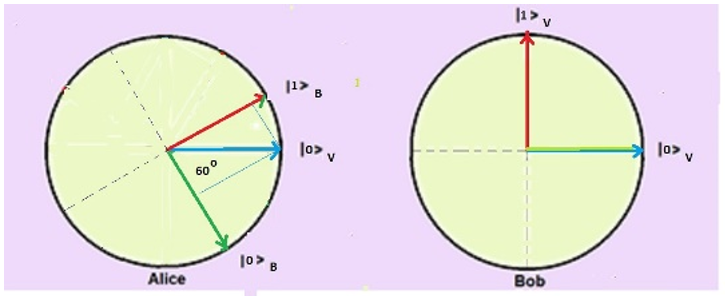
\includegraphics[width=.5\textwidth]{./img/opgbella.PNG}
\item P(rood bij Alice) = $\left(\tfrac{\sqrt{3}}{2}\right)^2= \tfrac{3}{4}$ (zie figuur)
\item P(groen  bij Alice) = $\left(\tfrac{1}{2}\right)^2= \tfrac{1}{4} $
\item P(rood  bij Bob) = 0 
\item P(groen  bij Bob) = 1
\item P(RG) =P(rood  bij Alice)* P(groen  bij Bob)= $\tfrac{3}{4}*1=\tfrac{3}{4}$. 
\item Eerste manier:\\
P(RR) =$\tfrac{3}{4}*0=0$\\
P(GG) =$\tfrac{1}{4}*1=\tfrac{1}{4}$\\
Dus kans op twee gelijke kleuren =$\tfrac{1}{4}$.

Tweede manier:\\
P(gelijke kleur)= 1 - P(verschillende kleur)= 1 – P(RG)-P(GR)=$\tfrac{1}{4}$

\end{enumerate}
\fi%=6-=-6


\subsection*{Hoofdstuk 3}

\textbf{opdr:brexit}~\ref{opd:lineair}

$y=3(5+6)=$\\$3*5+3*6=33$\\
$y=3(4*5)=$\\$4*3*5=60$


\textbf{opdracht}~\ref{opd:lineair2}%3.2

$\port{$Z$}\left(\alpha\ket{0}+\beta\ket{1}\right)  =$\\
$\port{$Z$}\alpha \ket{0}+\port{$Z$}\beta \ket{1}  = $\\
$\alpha \port{$Z$}\ket{0}+\beta \port{$Z$}\ket{1}$\\
met $\port{$Z$}\ket{0}=\ket{0}$ en $\port{$Z$}\ket{1}=\ket{-1}=-\ket{1}$: \\
$\alpha\ket{0}+\beta\ket{-1})   =  \smqty(\alpha\\ -\beta)$

\textbf{opdracht}~\ref{opd:toestanda}%3.3

\begin{enumerate}
\item tekenen
\item $\tfrac{\pi}{3}$= \SI{60}{\degree}
\item $\tfrac{1}{4}\sqrt{2}\mqty(1+\sqrt{3}\\ 1-\sqrt{3})$
\item $1$
\end{enumerate}



\begin{flushleft}
%\leavevmode
\begin{minipage}{.45\textwidth}
\def\ojfrangle{0}
\def\ojobangle{60}
\def\ojscale{.75}
\begin{tikzpicture}%
\begin{scope}[scale=\ojscale, rotate=\ojfrangle]
  \draw[thin,gray!40] (-0.1,-0.1) grid (5,5);
  \draw[-stealth] (-0.1,0)--(5*cos{\ojobangle},0) 
        node[midway, below, xshift=0]
        {${\scriptstyle{\alpha}}$};
%        {${\scriptstyle\braket{0}{\Psi}}$};
  \draw[-stealth] (0,-0.1)-- (0,5*sin{\ojobangle}) 
        node[midway, left, yshift=0]
        {${\scriptstyle{\beta}}$};
%        {${\scriptstyle\braket{1}{\Psi}}$};
  \node[above] at (0,5) {$\ket{1}$};
  \node[right] at (5,0) {$\ket{0}$};
  \draw[line width=.1pt ,black] ([shift=(0:5)]0,0) arc (0:90:5);
  \draw[thick, red, -stealth](0,0)--(90:5);
  \draw[thick, green, -stealth](0,0)--(0:5);
  \draw[thick, blue, -stealth](0,0)--(\ojobangle:5)
       node[label={[above, right]$\ket{\Psi}$}] (p){};
  \draw[line width=1pt,dotted] (0,5*sin{\ojobangle}) -- (p);
  \draw[line width=1pt,dotted] (p)--(5*cos{\ojobangle},0);
\end{scope}
\end{tikzpicture}
\end{minipage}%
\hfill
\begin{minipage}{.5\textwidth}
Hoek met de horizontaal: $\tan^{-1}\tfrac{\tfrac{1}{2}\sqrt{3}}{\tfrac{1}{2}}=\SI{60}{\degree}$
\begin{enumerate}
\item tekening
\item Hoek met de horizontaal: $\tan^{-1}\tfrac{\tfrac{1}{2}\sqrt{3}}{\tfrac{1}{2}}=\SI{60}{\degree}$
\item $\tfrac{1}{4}\sqrt{2}\mqty(1+\sqrt{3}\\ 1-\sqrt{3})$
\item $1$
\end{enumerate}
\end{minipage}
\end{flushleft}

Geheel analoog aan voorbeeld:
\[\begin{aligned}
\port{H}\Psi&=\port{H}(\frac{1}{2}\ket{0} +\frac{\sqrt{3}}{2}\ket{1})\\
&=\frac{1}{2}\port{H}\ket{0} +\frac{\sqrt{3}}{2}\port{H}\ket{1}\\
&=\frac{1}{2}\frac{1}{\sqrt{2}}\left(\ket{0}+\ket{1}\right)+\frac{\sqrt{3}}{2}\frac{1}{\sqrt{2}}\left(\ket{0}-\ket{1}\right))\\
&=\frac{\sqrt{2}}{4}(\ket{0}+\ket{1})+\frac{\sqrt{2}\sqrt{3}}{4}(\ket{0}-\ket{1})\\
&=\frac{\sqrt{2}}{4}((1+\sqrt{3})\ket{0}+(1-\sqrt{3})\ket{1})\\
\end{aligned}\]



\textbf{opdr:}~\ref{opd:diagstandaard}
\begin{enumerate}
\item
\[\begin{aligned}
\ket{0}&=\tfrac{1}{\sqrt{2}}\ket{+}+\tfrac{1}{\sqrt{2}}\ket{-}\\
\ket{1}&=\tfrac{1}{\sqrt{2}}\ket{+}-\tfrac{1}{\sqrt{2}}\ket{-}\\
\end{aligned}\]%[-2\baselineskip]
\item 
\[\begin{aligned}
\port{$H$}\ket{+}=\\
\port{$H$}\tfrac{1}{\sqrt{2}}(\ket{0}+\ket{1})=\\
\tfrac{1}{\sqrt{2}}\port{$H$}(\ket{0}+\ket{1})=\\
\tfrac{1}{\sqrt{2}}(\port{$H$}\ket{0}+\port{$H$}\ket{1})=\\
\tfrac{1}{\sqrt{2}}\left(\tfrac{1}{\sqrt{2}}(\ket{0}+\ket{1})+\tfrac{1}{\sqrt{2}}(\ket{0}-\ket{1})\right)=\\
\ket{0}
\end{aligned}\]%[-2\baselineskip]
\end{enumerate}


\textbf{exp werkblad QI}~\ref{sec:wbQI} Hiervan is geen uitwerking

\textbf{exp kopofmunt} (uitgewerkt in lessenplan~\ref{sec:kopofmunt})

\textbf{opdr:}~\ref{opd:Ry30Ry30}%3.5

\[\begin{aligned}
&\port{Ry30}(\port{Ry30}(\ket{0})\\
&=\port{Ry30}(\tfrac{1}{2}\sqrt{3}\ket{0}+\tfrac{1}{2}\ket{1})\\
&=\tfrac{1}{2}\sqrt{3}\port{Ry30}\ket{0}+\tfrac{1}{2}\port{Ry30}\ket{1})\\
&=\tfrac{1}{2}\sqrt{3}\left(\tfrac{1}{2}\sqrt{3}\ket{0}+\tfrac{1}{2}\ket{1}\right)+\tfrac{1}{2}\left(-\tfrac{1}{2}\ket{0}+\tfrac{1}{2}\sqrt{3}\ket{1}\right)\\
&=\tfrac{3}{4}\ket{0}+\tfrac{\sqrt{3}}{4}\ket{1}-\tfrac{1}{4}\ket{0}+\tfrac{\sqrt{3}}{4}\ket{1}\\
&=\tfrac{1}{2}\ket{0} +\tfrac{1}{2}\sqrt{3}\ket{1}
\end{aligned}\]
En dat is precies een draaiing over \SI{60}{\degree}


\textbf{opdr:}~\ref{opd:XICNOT}%3.6

\begin{tabular}{|l|l|l|}
\hline
input& T \quad & output\\ \hline
$\ket{00}$ &$\ket{00}$ & $\ket{00}$ \\ \hline %\cline{1-2}% \cline{4-5} 
$\ket{01}$ &$\ket{10}$ & $\ket{11}$ \\ \hline %\cline{1-2}% \cline{4-5} 
$\ket{10}$ &$\ket{01}$ & $\ket{01}$ \\ \hline %\cline{1-2}% \cline{4-5} 
$\ket{11}$ &$\ket{11}$ & $\ket{10}$ \\ \hline %\cline{1-2}% \cline{4-5} 
\end{tabular}

\textbf{opdr:}~\ref{opd:CNOTterug}%3.7

\begin{tabular}{|l|l|}
\hline
input& output\\ \hline
$\ket{00}$&$\ket{00}$ \\ \hline %\cline{1-2}% \cline{4-5} 
$\ket{10}$&$\ket{01}$ \\ \hline %\cline{1-2}% \cline{4-5} 
$\ket{11}$&$\ket{10}$ \\ \hline %\cline{1-2}% \cline{4-5} 
$\ket{01}$&$\ket{11}$ \\ \hline %\cline{1-2}% \cline{4-5} 
\end{tabular}

\textbf{opdr:}~\ref{opd:verstrengeling}%3.8

\begin{enumerate}[wide, labelwidth=!, labelindent=0pt]
\item
$\port{H}\ket{0}\ket{0}=$\\
$\tfrac{1}{\sqrt{2}}\left(\ket{0}+\ket{1}\right)\ket{0}=$\\
$\tfrac{1}{\sqrt{2}}\ket{00}+\tfrac{1}{\sqrt{2}}\ket{10}$
\item $\tfrac{1}{\sqrt{2}}\port{CNOT}\left(\ket{00}+\ket{10}\right)$=
$\tfrac{1}{\sqrt{2}}\left(\ket{00}+\ket{11}\right)$

\item Nee, niets is buiten haakjes te halen
\item I. NB $\alpha=\beta=\tfrac{1}{2}\sqrt{2}$
\item $\ket{00} \implies I$\\
$\ket{10}\implies II$\\
$\ket{01}\implies III$\\
$\ket{11}\implies IV$
\end{enumerate}


\textbf{opdr:}~\ref{opd:ry30cnot}%3.9
%NB 0.71=$\tfrac{1}{\sqrt{2}}$
\begin{enumerate}
\item
\hspace{3cm}\begin{minipage}{0.5\textwidth}
\Qcircuit @C=.5em @R=2em {
\lstick{Alice:~q_0 = \ket{0}} \ar@{.}[]+<0.5em,1em>;[d]+<0.5em,-1em>& \qw  & \gate{H} \ar@{.}[]+<2em,1em>;[d]+<2em,-1em>   &\qw  & \qw &\ctrl{1} & \qw & \ar@{.}[]+<0em,1em>;[d]+<0em,-1em>\qw  & \qw   & \meter \ar@{.}[]+<0em,-0.5em>;[d]+<0em,-1em> & \ar@{.}[d]+<0em,-0.5em>;[d]+<0em,-1em>\\
\lstick{Bob:~q_1 = \ket{0}}   & \qw             & \gate{Ry30} &\qw             & \qw &\targ    & \qw & \qw             &\qw    & \qw          & \meter\\
                              &\ustick{t_0}     &             &\ustick{t_1}    &     &         &     & \ustick{t_2}    &       & \ustick{t_3} & \ustick{t_4} 
}
\end{minipage}
\hfill
\item De toestand op $t_2$ wordt nu:

$\port{CNOT}\tfrac{1}{\sqrt{2}}\left(\ket{0}+\ket{1}\right)\left(\tfrac{1}{2}\sqrt{3}\ket{0}+\tfrac{1}{2}\ket{1}\right)=$

$\sqrt{\tfrac{3}{8}}\ket{00}+
 \sqrt{\tfrac{1}{8}}\ket{01}+
 \sqrt{\tfrac{1}{8}}\ket{10}+
 \sqrt{\tfrac{3}{8}}\ket{11}$

\item Verschillende kleuren als 
\end{enumerate}


\textbf{opdr:}~\ref{opd:ry60cnot}%3.10
\begin{enumerate}
\item De toestand op $t_1$:\\
$\port{H}\ket{0}\otimes\port{Ry60}\ket{0}=$\\
$\tfrac{1}{\sqrt{2}}\left(\ket{0}+\ket{1}\right)\otimes\left(\tfrac{1}{2}\ket{0}+\tfrac{1}{2}\sqrt{3}\ket{1}\right)=$\\
$\sqrt{\tfrac{1}{8}}\ket{00}+
 \sqrt{\tfrac{3}{8}}\ket{01}+
 \sqrt{\tfrac{1}{8}}\ket{10}+
 \sqrt{\tfrac{3}{8}}\ket{11}$

\item 
\[\begin{aligned}\sqrt{\tfrac{1}{8}}\ket{00}+\sqrt{\tfrac{3}{8}}\ket{01}+\sqrt{\tfrac{3}{8}}\ket{10}+\sqrt{\tfrac{1}{8}}\ket{11}\end{aligned}\]
\item De termen 3 en 4 vallen af. Blijft over $\tfrac{1}{2}\ket{00}+\tfrac{1}{2}\sqrt{3}\ket{01}$
\item Kans dat Bob een 0 meet (in vervolg op vorige vraag) = ${\tfrac{1}{2}}^2=\tfrac{1}{4}$
\item 
\begin{tabular}{|r|c|c|}
\hline
         & $B_{0}$          & $B_{1}$ \\ \hline
$A_{0}$  &   $\tfrac{1}{4}$ &  $\tfrac{3}{4}$ \\ \hline
$A_{1}$  &   $\tfrac{1}{4}$ &  $\tfrac{3}{4}$ \\ \hline
\end{tabular}
\item De termen 2 en 4 vallen af. Blijft over $\tfrac{1}{2}\ket{00}+\tfrac{1}{2}\sqrt{3}\ket{10}$
\item wederom ${\tfrac{1}{2}}^2=\tfrac{1}{4}$
\item De tabel blijft ongewijzigd. Bob meet als eerste en heeft nu $\tfrac{1}{2}$ kans op 
nul, (meest rechtse kolom in de tabel. Alice heeft $\tfrac{1}{4}$ kans op nul.
\end{enumerate}

\textbf{opdr:}~\ref{opd:ryonbekend}%3.11
\begin{enumerate}
\item 
$\tfrac{1}{2}\alpha^2=0.201,\alpha \approx \sqrt{0.408}\approx 0.639$\\
$\tfrac{1}{2}\beta^2=0.291,  \beta \approx \sqrt{0.592}\approx 0.769$\\
$\tfrac{1}{2}\beta^2=0.301,  \beta \approx \sqrt{0.592}\approx 0.769$\\
$\tfrac{1}{2}\alpha^2=0.207,\alpha \approx \sqrt{0.408}\approx =0.639$\\
check: $\alpha^2+\beta^2=0.408+0.592=1$, =ok

\item 
\begin{flushleft}
%\leavevmode
\begin{minipage}{.45\textwidth}
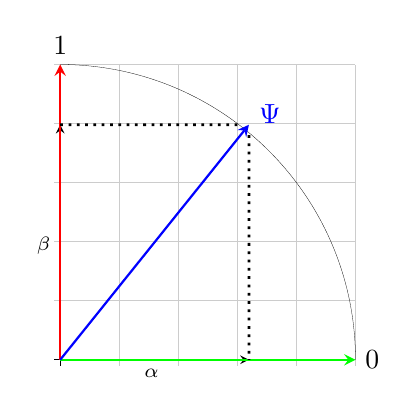
\begin{tikzpicture}%
\def\a{0.639}
\def\b{0.796}
\def\ojfrangle{0}
%\def\ojobangle{atan{\b/\a}}
\def\ojscale{.75}
\begin{scope}[scale=\ojscale, rotate=\ojfrangle]
  \draw[thin,gray!40] (-0.1,-0.1) grid (5,5);
  \draw[-stealth] (-0.1,0)--(5*\a, 0)%                   cos{\ojobangle},0) 
        node[midway, below, xshift=0]
        {${\scriptstyle{\alpha}}$};
  \draw[-stealth] (0,-0.1)-- (0,5*\b)%                sin{\ojobangle}) 
        node[midway, left, yshift=0]
        {${\scriptstyle{\beta}}$};
  \node[above] at (0,5) {$\ket{1}$};
  \node[right] at (5,0) {$\ket{0}$};
  \draw[line width=.1pt ,black] ([shift=(0:5)]0,0) arc (0:90:5);
  \draw[thick, red, -stealth](0,0)--(90:5);
  \draw[thick, green, -stealth](0,0)--(0:5);
  \draw[thick, blue, -stealth](0,0)--(5*\a, 5*\b)
       node[label={[above, right]$\ket{\Psi}$}] (p){};
  \draw[line width=1pt,dotted] (0,5*\b) -- (p);
  \draw[line width=1pt,dotted] (p)--(5*\a,0);
\end{scope}
\end{tikzpicture}
\end{minipage}%
\end{flushleft}


\item De hoek kan uit de figuur bepaald worden of berekend met  $tan^{-1}\tfrac{\beta}{\alpha} \approx \SI{50}{\degree} (0.28 \pi rad)$. 


Hier een wat uitgebreider antwoord. Enkele simulaties op QI leveren het volgende resultaat.

\begin{flushleft}
\small{
\begin{tabular}{|r|l|l|l|l||l|l|}
\hline
$\theta=$     & 0=$\ket{00}$  & 1=$\ket{01}$   & 2=$\ket{10}$   & 3=$\ket{11}$ &$\alpha^2$&$\beta^2$ \\ \hline
$0$           & 0.475 &        &        & 0.5244 & 1 &0 \\
$\pi/6=0.523$ & 0.472 & 0.027  & 0.038  & 0.4619 &   & \\
$\pi/4=0.785$ & 0.418 & 0.079  & 0.065  & 0.4365 & & \\
$\pi/3=1.04$  & 0.354 & 0.129  & 0.125  & 0.3876 & & \\
$\pi/2=1.57$  & 0.240 & 0.240  & 0.254  & 0.2646 & 0.5&0.5 \\
$7\pi/12=1.83$& 0.188 & 0.312  & 0.310  & 0.191  & & \\
$2\pi/3=2.08$ & 0.115 & 0.400  & 0.372  & 0.112  & & \\
$\pi=3.14$    &       & 0.511  & 0.482  &        &0 &1 \\
$opgave$      & 0.201 & 0.291  & 0.301  & 0.207  &0.408 & 0.592 \\
\hline
\end{tabular}
}
\end{flushleft}

Uit de simulaties volgt bijvoorbeeld: Bij $\pi/2$ is $\alpha^2=\beta^2=\tfrac{1}{2}$. 
In ons co\"ordinatenstel levert dat \SI{45}{\degree}, \textbf{Bij QI zijn de hoeken twee keer zo groot}: \SI{90}{\degree} ($\tfrac{\pi}{2}$)

\item Je berekent de hoek met de getallen van de opgave:\\
 $2*\arctan\tfrac{0.796}{0.639}\approx 1.79 rad $


\item Mijn antwoord wijkt wel erg af:
\begin{flushleft}
\small{
\begin{tabular}{|r|l|l|l|l||l|l|}
\hline
$\theta=$     & 0=$\ket{00}$  & 1=$\ket{01}$   & 2=$\ket{10}$   & 3=$\ket{11}$ &$\alpha^2$&$\beta^2$ \\ \hline
$0.55\pi=1.75$ & 0.188 & 0.295  & 0.306  & 0.212 &   & \\
\hline
\end{tabular}
}
\end{flushleft}

\end{enumerate}




\section{Uitwerking werkbladen}\label{sec:uitwerkbladen}

De meeste zijn al beschreven in sectie~\ref{sec:lessenplan}. 


\paragraph*{werkblad Klassieke bits}

Klassieke bits bestuur je met klassieke poorten. Dit werkbablad gaat over Boolse algebra en bis die per se 1 of 0 zijn. 

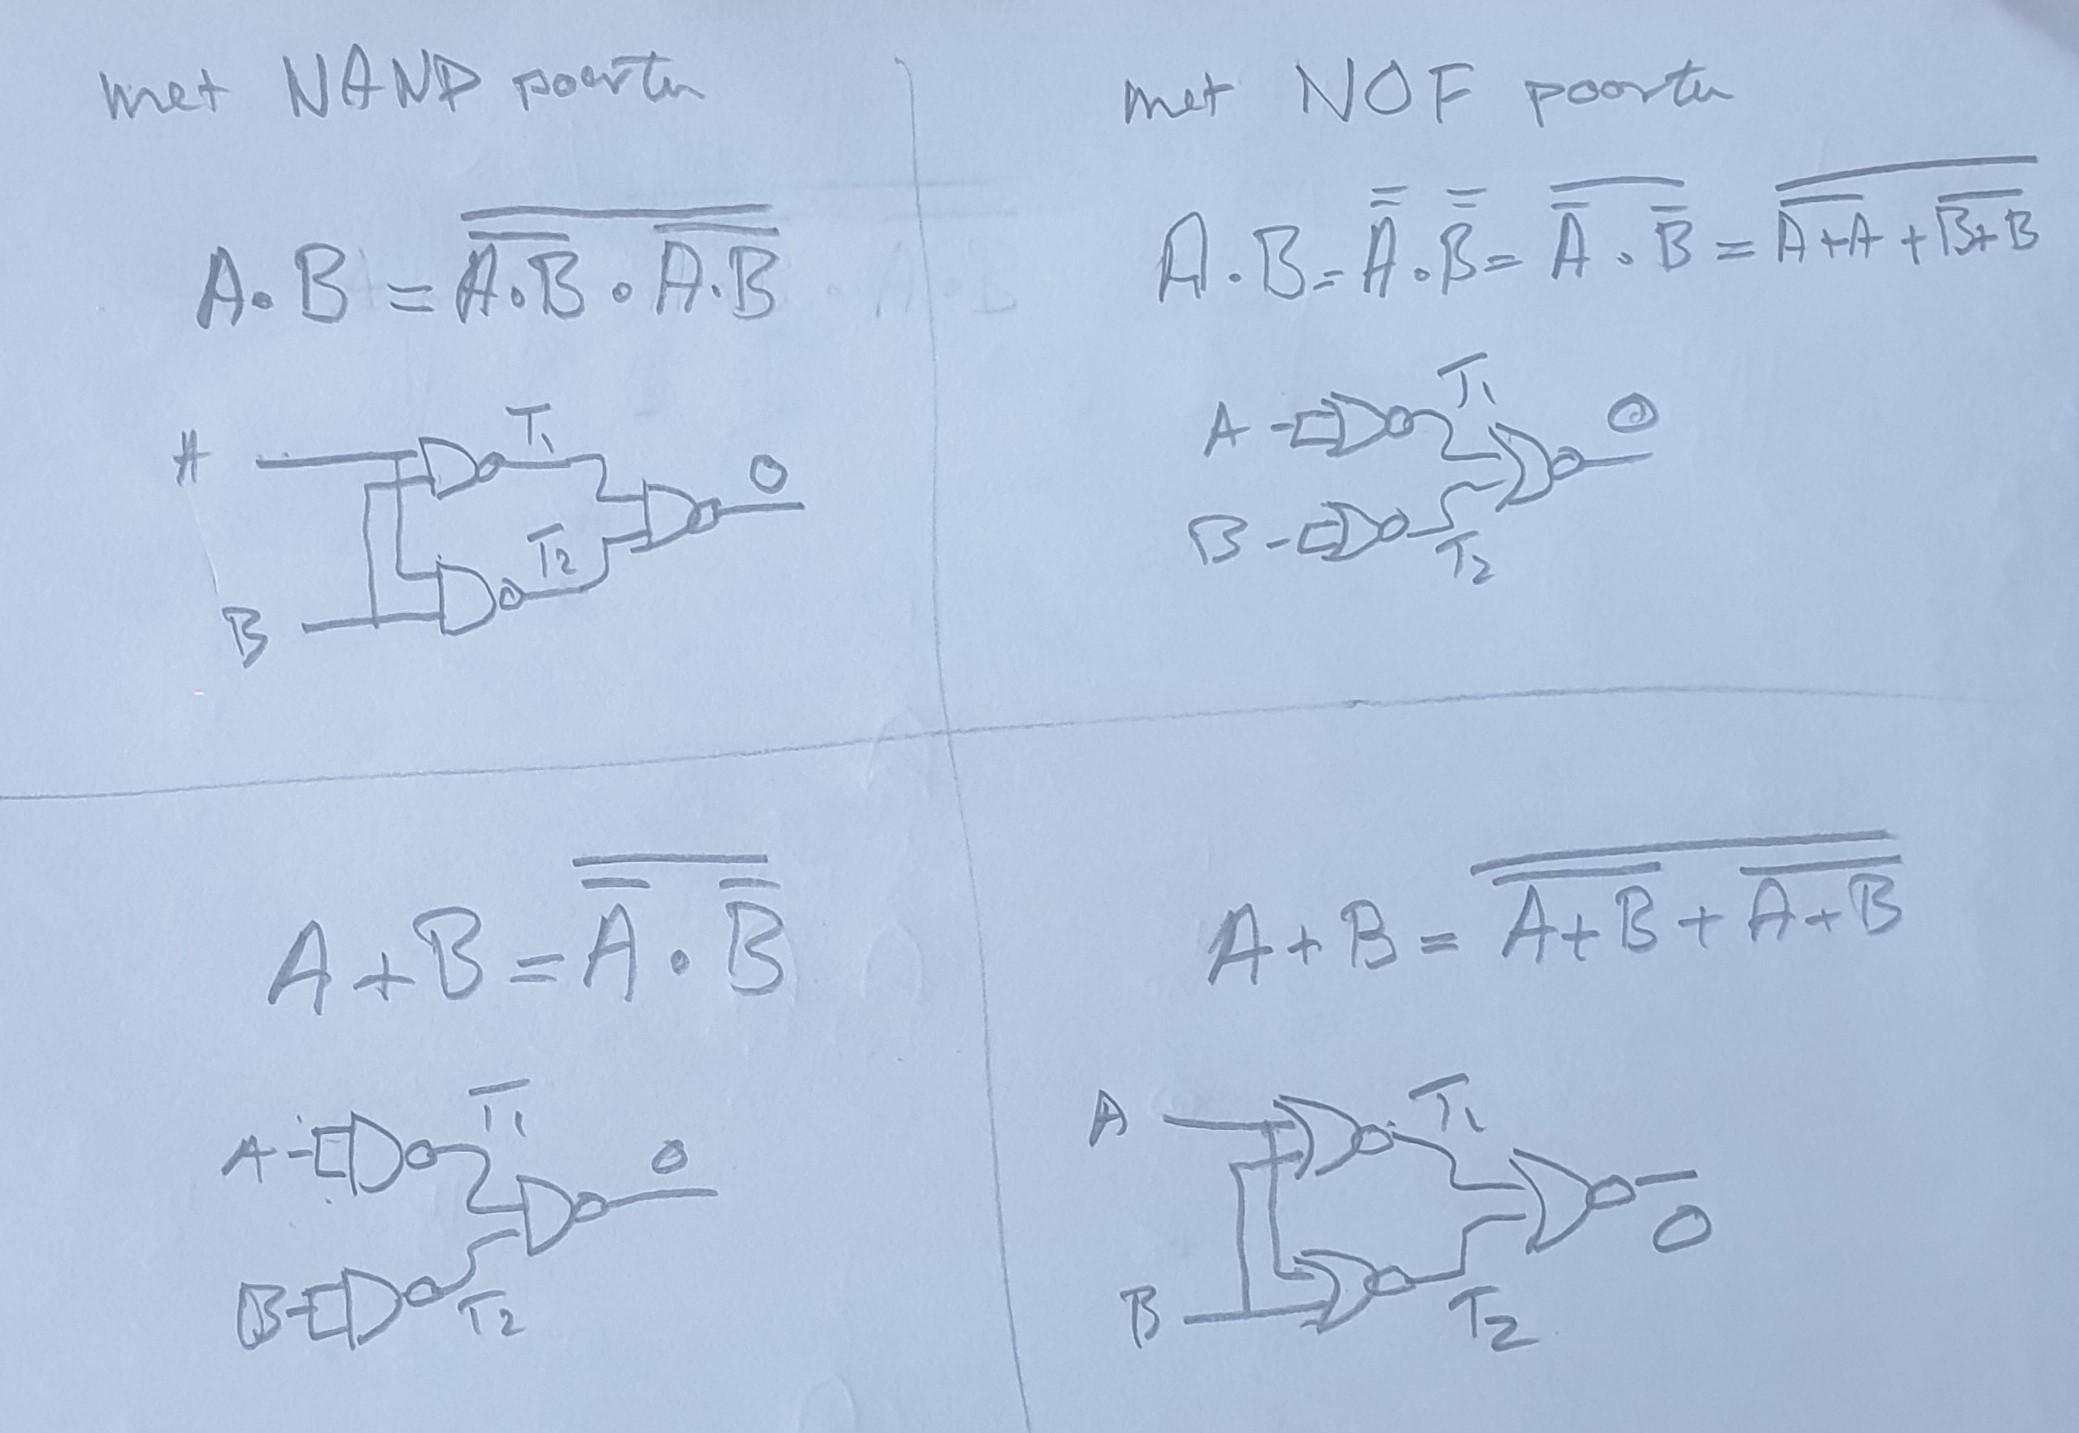
\includegraphics[width=\textwidth]{./img/klassiekuitwerking.jpg}

Als voorbeeld de waarheidtabel van $A \cdot B$ uitgedrukt in NEN poorten

\[ A \cdot B= \overline{\overline{{A} \cdot {B}}} = \overline{\overline{A \cdot B} \cdot \overline{A \cdot B}}\]

\begin{tabular}{|l|l|l|l|l|}
\hline
$A$ & $B$ & $T_1$ &$T_2$& $O$\\ \hline
0     & 0     & 1 &  1  &  0 \\ \hline
0     & 1     & 1 &  1  &  0 \\ \hline
1     & 0     & 1 &  1  &  0 \\ \hline
1     & 1     & 0 &  0  &  1 \\ \hline
\end{tabular}

\paragraph*{werkblad Teleportatie}

Werkblad teleportatie kunnen leerlingen zelf het protocol afleiden. Niet moeilijk, wel secuur werk, niet alle leerlingen gaan dit volbrengen. Gelukkig staat het antwoord achteraan.

Losse vragen:

a)c\\
b)b\\
c)Nee, Je meet een toestand $\ket{0}$ met een kans $\alpha^2$ of $\ket{1}$ met kans $\beta^2$.\\
d)Je kunt de toestand telkens opnieuw bouwen en het kansproces herhalen. Zo kun je uiteindelijk de co\"effici\"enten benaderen. die gelden tot het qubit gemeten wordt.

e)I, f)X, g)Z, h)XZ

Hier staat het protocol helemaal uitgeschreven.



Hoe werkt het teleportatieprotocol nou precies?

\paragraph*{$t_0$} We beginnen met een qubit $T=\alpha\ket{0}+\beta\ket{1}$, en Alice en Bob hebben allebei een qubit in toestand $\ket{0}$. Met het tensorproduct kunnen we ze schrijven als
\[\ket{T}\otimes\ket{A}\otimes\ket{B}=\ket{TAB} = \left(\alpha\ket{0}+\beta\ket{1}\right)\ket{00}= \alpha\ket{000}+\beta\ket{100}\]
\paragraph*{$t_1$} Als eerste wordt qubit A door een \port{H}-poort geleid:
\[\begin{aligned}
T &\otimes \port{H}\ket{A}\ket{0_B} =\\
T &\otimes \frac{\ket{0_A}+\ket{1_A}}{\sqrt{2}}\ket{0_B} =\\
\left(\alpha\ket{0_T}+\beta\ket{1_T}\right) &\otimes \left(\frac{1}{\sqrt{2}}\ket{0_A0_B}+\frac{1}{\sqrt{2}}\ket{1_A0_B}\right)
\end{aligned}\]

Deze toestand kunnen we ook opschrijven door de haakjes weg te werken als:
\[\begin{aligned}
\frac{\alpha}{\sqrt{2}}\ket{0_T0_A0_B} +
\frac{\alpha}{\sqrt{2}}\ket{0_T1_A0_B} +
\frac{\beta}{\sqrt{2}}\ket{1_T0_A0_B} +
\frac{\beta}{\sqrt{2}}\ket{1_T1_A0_B}
\end{aligned}\]

\paragraph*{$t_2$} Alice past een \port{CNOT}-poort toe op A en B. A is hierbij het controlebit en B het doel. Een CNOT laat het doel onveranderd als het controlebit 0 is, en flipt het doel als het controlebit 1 is. Bob gaat op reis en neemt zijn register mee.

\[\begin{aligned}
\frac{\alpha}{\sqrt{2}}\ket{0_T0_A0_B} +
\frac{\alpha}{\sqrt{2}}\ket{0_T1_A1_B} +
\frac{\beta}{\sqrt{2}}\ket{1_T0_A0_B} +
\frac{\beta}{\sqrt{2}}\ket{1_T1_A1_B}
\end{aligned}\]

\paragraph*{$t_3$} Alice past een \port{CNOT}-poort toe op haar twee qubits met T als controlebit en A als doel. 

\[\begin{aligned}
\frac{\alpha}{\sqrt{2}}\ket{0_T0_A0_B} +
\frac{\alpha}{\sqrt{2}}\ket{0_T1_A1_B} +
\frac{\beta}{\sqrt{2}}\ket{1_T1_A0_B}  +
\frac{\beta}{\sqrt{2}}\ket{1_T0_A1_B}
\end{aligned}\]

\paragraph*{$t_4$}Daarna voert Alice het qubit dat ze wil teleporteren, $T$, door een Hadamard-poort. Dit levert:

\[\begin{aligned}
\frac{\alpha}{2}(\ket{0_T}+\ket{1_T})\ket{0_A0_B} &+
\frac{\alpha}{2}(\ket{0_T}+\ket{1_T})\ket{1_A1_B} +\\
\frac{\beta}{2}(\ket{0_T}-\ket{1_T})\ket{1_A0_B} &+ 
\frac{\beta}{2}\ket{0_T}-\ket{1_T})\ket{0_A1_B}
\end{aligned}\]

We schrijven de toestand hierboven zo dat de twee qubits van Alice samen staan. Dit doen we in twee stappen. Eerst zullen we de toestand buiten haakjes halen (acht termen):

\[\begin{aligned}
\frac{\alpha}{2}\ket{0_T0_A0_B} + \frac{\alpha}{2}\ket{1_T0_A0_B} &+ 
\frac{\alpha}{2}\ket{0_T1_A1_B} + \frac{\alpha}{2}\ket{1_T1_A1_B} +\\
\frac{\beta}{2}\ket{0_T1_A0_B} - \frac{\beta}{2}\ket{1_T1_A0_B} &+
\frac{\beta}{2}\ket{0_T0_A1_B} - \frac{\beta}{2}\ket{1_T0_A1_B}
\end{aligned}\]

Wanneer we Alice's qubits apart opschrijven van Bob's qubits, krijgen we de toestand:

\[\begin{aligned}
\frac{\alpha}{2}\ket{0_T0_A}\ket{0_B} +\frac{\alpha}{2}\ket{1_T0_A}\ket{0_B} &+\frac{\alpha}{2}\ket{0_T1_A}\ket{1_B} +\frac{\alpha}{2}\ket{1_T1_A}\ket{1_B} +\\
\frac{\beta}{2}\ket{0_T1_A}\ket{0_B} -\frac{\beta}{2}\ket{1_T1_A}\ket{0_B} &+\frac{\beta}{2}\ket{0_T0_A}\ket{1_B} -\frac{\beta}{2}\ket{1_T0_A}\ket{1_B}
\end{aligned}\]

En door nu termen buiten haakjes te halen, krijgen we:

\[\begin{aligned}
\frac{1}{2}\ket{0_T0_A}(\alpha\ket{0_B}+\beta\ket{1_B}) +\frac{1}{2}\ket{1_T0_A}(\alpha\ket{0_B} &- \beta\ket{1_B}) +\\
\frac{1}{2}\ket{0_T1_A}(\alpha\ket{1_B} + \beta\ket{0_B}) +\frac{1}{2}\ket{1_T1_A}(\alpha\ket{1_B} &- \beta\ket{0_B})\\
\end{aligned}\]


Het enige wat Alice nu nog hoeft te doen is haar twee qubits meten. Zoals je ziet, geeft elke mogelijke meetuitkomst van haar twee qubits, een andere toestand van de qubits van Bob. Zoals je kunt zien, zal Bob de originele toestand van $T$ meten, wanneer Alice $\ket{00}$ meet. Maar ook wanneer Alice niet $\ket{00}$ meet, kan Bob de originele toestand terugkrijgen door een simpele enkele qubit poort toe te passen. Het enige wat Bob niet weet, is wat Alice's meetuitkomst is. Daarom moet Alice, nadat ze gemeten heeft, haar toestand doorgeven aan Bob via een klassiek kanaal. Dit kan via de telefoon, via e-mail, of hoe ze ook wil. Daarna weet Bob precies wat hij moet doen. Meet Alice $\ket{00}$? Dan meet Bob zijn qubit en weet hij $T$. Meet Alice $\ket{01}$, dan heeft Bob de toestand $\alpha\ket{1_B} + \beta\ket{0_B}$. Wanneer hij dan een X-poort op zijn qubits toepast, verandert de toestand in $\alpha\ket{0_B} + \beta\ket{1_B}$ en dit is weer precies $T$. Wanneer Alice $\ket{10}$ meet, dan heeft Bob de toestand $\alpha\ket{0_B} - \beta\ket{1_B}$. Wanneer hij nu een Z-poort toepast, dan wordt zijn qubit: $\alpha\ket{0_B} + \beta\ket{1_B}$ en heeft hij weer $T$.

\begin{enumerate}[start=9]
\item Bob's qubit is instantaan vastgelegd als Alice meet. Echter ze moet Bob eerst opbellen (klassiek kanaal) om haar resultaat door te geven. Dat gaat niet sneller dan het licht.
\item Een lamp is geen quantumobject,  laat staan dat een persoon dat is.  Vraag is natuurlijk of het theoretisch verboden is, dat niet.
\item Dat gaat ook maar met een andere decodering. Dus wel afspraken maken vooraf.
\end{enumerate}

Om over na te denken: Alice heeft twee complexe co\"effici\"enten getransoprteerd naaar Bob geteleporteerd. Dat heeft ze gedaan door twee klassieke bits door te bellen.
Hoe zijn die $\alpha$en  $\beta$ nu overgedragen? Dit is de kracht van verstrengeling.


\iffalse%----nog uitwerken----
nog wat extra opdrachten bij teleportatie}

\begin{antwoord}
\end{antwoord}
\begin{opdracht}
\begin{enumerate}
\item Laat zien dat, als qubit $T$ in de toestand 
\[\ket{\Psi}=a\ket{0}+b\ket{1}\] 
zit, de de totale toestand van het systeem kunt schrijven als
\begin{align*}
\psi_0\rangle=\frac{1}{\sqrt{2}}\left[a (|001\rangle + |010\rangle) + b (|101\rangle +|110\rangle)\right],
\end{align*}
waarbij de eerste twee qubits dus van Alice zijn en de laatste van Bob.

\item We passen nu een \port{CNOT} gate toe op de qubits van Alice, waarbij de eerste qubit de control is en de tweede het doel. Laat zien dat je de toestand nu kunt schrijven als
\begin{align*}
|\psi_1\rangle=\frac{1}{\sqrt{2}}\left[a (|001\rangle + |010\rangle) + b (|111\rangle +|100\rangle)\right]
\end{align*}

\item Zoals je kunt zien in de afbeelding is de volgende stap dat we de eerste qubit door een Hadamard gate laten gaan. Laat zien dat hierdoor de volgende toestand ontstaat:
\begin{align*}
|\psi_2\rangle=\frac{1}{2}\left[a (|0\rangle +|1\rangle)(|01\rangle + |10\rangle) + b (|0\rangle - |1\rangle)(|11\rangle +|00\rangle)\right]
\end{align*}

\item Laat nu zien dat deze toestand om te schrijven is tot
\begin{align*}
|\psi_2\rangle=\frac{1}{2}&\big[ |00\rangle(a|1\rangle + b |0\rangle) \\
+& |01\rangle (a|0\rangle + b|1\rangle) \\
+&|10\rangle(a|1\rangle - b|0\rangle) \\
+ &|11\rangle (a|0\rangle - b|1\rangle) \big]
\end{align*}
\end{enumerate}
\end{opdracht}
Dit is een hele interessante toestand. Wanneer Alice nu haar twee qubits meet en haar resultaat via een klassiek kanaal naar Bob verstuurt, weet Bob precies in welke toestand zijn qubit zit (aannemende dat hij weet wat Alice heeft gedaan met haar qubits). Als Alice $|00\rangle$ meet, hoeft Bob niks meer te doen en heeft hij al de juiste toestand voor zijn qubit. Voor de andere drie gevallen moet hij echter nog wat werk doen.

\begin{antwoord}
\end{antwoord}
\begin{opdracht}
\begin{enumerate}
\item Wat kan Bob doen om de juiste toestand te krijgen als hij van Alice te horen krijgt dat ze $|10\rangle$ heeft gemeten?
\item En wat moet hij doen als ze $|01\rangle$ heeft gemeten?
\item Combineer je antwoorden van e) en f) om erachter te komen wat hij moet doen als Alice $|11\rangle$ heeft gemeten.
\item Heeft Alice nog steeds de toestand $|\psi\rangle$? Was dit te verwachten aan de hand van wat je eerder vandaag hebt gehoord?
\item [Bonus] Heb je tijd over of nog niet genoeg gehad van quantumteleportatie? Kijk dan of dit algoritme ook werkt voor (\'e\'en van) de andere Bell toestanden.
\end{enumerate}
\end{opdracht}


H5
 Quantumcomputers maken gebruik van meer dan \'e\'en qubit. De rekenkracht van een quantumcomputer stijgt \textit{exponentieel} met het aantal qubits.

extra oefenen met registers (\ref{sec:registers})

Invoer en uitvoer worden bij een register weergegeven als een rijtje. De invoer in fig.~\ref{fig:algo2b1x} bijvoorbeeld wordt dan weergegeven als $\ket{0}$,$\ket{0}$  of kortweg als $\ket{00}$.  Daarbij lezen we het rijtje van links naar rechts. De eerste qubit komt in deze conventie overeen met de bovenste lijn in de grafische presentatie.  (sommige bronnen doen dit net andersom, dus altijd even opletten!)
\begin{antwoord}
\begin{itemize}
  \item $\ket{0}$, immers geflipped door \port{CNOT}
  \item $\alpha=\frac{4}{\sqrt{5}},\newline \beta=\frac{3}{\sqrt{5}}$
\end{itemize}
\end{antwoord}
\begin{opdracht}\label{opdr:xztabel}
Voor eenvoudige circuits kan een input-output tabel worden gemaakt. Maak zo'n tabel voor het onderstaande circuit.
\newline
\vspace{0.25cm}
%\begin{center}
%\leavevmode
\hspace{34pt}
\begin{minipage}{0.4\textwidth}
\Qcircuit @C=1em @R=2em {
\ustick{q[0]}&\qw & \gate{X}  & \qw \\
\ustick{q[1]}&\qw & \gate{Z}  & \qw\\ 
}
\end{minipage}
\hfill
\begin{minipage}{0.4\textwidth}
\begin{tabular}{|l|l|l|}
\hline
input&  output\\ \hline
$\ket{00}$  & \\ \hline %\cline{1-2}% \cline{4-5} 
$\ket{01}$  & \\ \hline %\cline{1-2}% \cline{4-5} 
$\ket{10}$  & \\ \hline %\cline{1-2}% \cline{4-5} 
$\ket{11}$  & \\ \hline %\cline{1-2}% \cline{4-5} 
\end{tabular}
\end{minipage}
%\end{center}
%\vspace{.5cm}
\end{opdracht}


meting: levert altijd een basistoestand! oefenvraag opnemen
  
\paragraph{Ondersteunende website}


bronvermeldingen
inspirerend materiaal 
referenties

\section{experimenten}

\subsection{Exp Interferentie met geluid}
Een toongenerator uit het natuurkundekabinet kan natuurljik, maar de laptop heeft het allemaal aan boord. Google (online tone generator, mei 2020) levert een link naar een \hrefqr{https://www.szynalski.com/tone-generator/}{webapplicatie}.

Stel de toongenerator in op ongeveer \SI{4}{\kilo\hertz}, niet te hard, de jonge oren zijn gevoelig. E\'en speaker aansluiten. Door de weerkaatsingen tegen de muur ontstaat er een staande golf patroon. Een oor afdoppen met je vinger zodat er \'e\'en 'microfoon' overblijft en het geluid beter gelokaliseerd kan worden. Beweeg je hoofd langzaam heen en weer en zoek de stilste plek op. Je kunt plekjes vinden waar het helemaal geen last hebt van die irritante toon.

\subsection{Rowili}
Is politiejargon voor rood-wit-lint. de prijs van Rowili is gestegen in de coronacrisis, met rol van 500 m kun je voorlopig vooruit,. Er is ook Gewili. Pas op koop niet de schuine strepen.  Google (aug 2020), afzetlint) 10-20 euro per 500 m

\subsection{Interferentie experimenten met licht}
We gebruiken een aantal demonstratie experimenten om de fysische begrippen interferentie en superpositie te illustreren.
De opstelling daarvoor is mogelijk te maken met spullen uit het kabinet, maar er is ook een kit beschikbaar. We gebruiken daarvoor een opstelling. 

citeer ross \cite{ross2020computer} : abstract QC shift in universitair onderwijs. Natuurlijk vanuit first principles op te bouwen, voor een klein aantal natuurkunde studenten..
Insteek kan ook zonder planck's constante en foto-electrisch effect. Inzicht in QC mogelijk zonder kennis vooraf uit de natuurkunde.
De introductie op de Dirac notatie is intensieve maar goede investering

We komen niet toe aan een formele aanpak.  begrippen als eigenwaarde, eigenvector unitair hebben we neit behandeld.
 
We maken een voorzichtig begin met \textit{augmented learning}. 


par 2.3
Wellicht een aparte opgave van maken?
\begin{enumerate}
\item Hoeveel pixels heeft het plaatje?
\item Hoeveel moleculen in een pixel?
\item Hoeveel atomen in een pigmentmolecuul? 
\item Hoeveel machten van tien verwijderd van een quantumtoestand?
\end{enumerate}

\textbf{Hoofdstuk 2}

De eerste logische poort werd door Rossi~\cite{rossi1930method} ontwikkeld voor het bestuderen van co\"inidenties van stralingsgebeurtenissen. Een AND poort met drie ingangen.

Correctie Eccles and Jordan patenteerden in 1918 de  \hrefqr{https://www.historyofinformation.com/detail.php?id=3606}{flipflip}

Wij willen niet te lang bij klassieke computers stilstaan. Het is een valkuil om in deze module te veel bij het hoofdstuk fysische infdormatica te blijven staan. Het gaat ons er om de essenti\"ele verschillen  in computerarchitectuur duidelijk te maken. 

We sommen enkele eigenschappen van klassieke computers op waar nu of later in de module verschillen met quantumcomputers uit kunnen worden afgeleid. 

De architectuur van de computer is in de veertiger jaren opgesteld.
Een aardig \hrefqr[-2cm]{https://www.futurelearn.com/courses/how-computers-work/0/steps/49284}{filmpje} van 4 minuten over de von Neumann Architectuur. Hierin wordt een berekening uitgevoerd die op jouw computer makkelijk binnen enkele nanoseconden wordt uitgevoerd.

\paragraph{klassieke poorten}
Een werkblad van een les over klassieke logica. We bieden een verdieping aan om een minimal set te definieren.


Uitleg minimal set met NAND gates (engelstalig):
\hrefqr[-2cm]{https://www.youtube.com/watch?v=2gLtCONHFtU&ab_channel=JacobSchrum}{uitleg}

Hier een overzicht van poorten
\hrefqr{https://www.electronics-tutorials.ws/logic/universal-gates.html}{universal logic gates}


Een geheugen in een klassieke computer.
\paragraph{Geheugen}


Door de uitgang terug te voeren naar de ingang kunnen we een geheugenelement maken, de flip-flop. Dit is de bouwsteen van het geheugen van een klassieke computer. 


\begin{tikzpicture}[thick]
 
% AND logic gates
\node (and1) at (0,2) {R};
\node (and2) at (0,-2) {S};
 
% NOR logic gates
\draw (and1) -- ++(2.5,0) node[ieeestd nand port, fill=cyan,anchor=in 1] (nor1) {};
\draw (and2) -- ++(2.5,0) node[ieeestd nand port, fill=cyan,anchor=in 2] (nor2) {};
 
\draw (nor1.in 2) -| ++ (-0.2,-0.85) -- ++(3,-1.5) coordinate(a) |- (nor2.out);
\draw (nor2.in 1) -| ++ (-0.2,0.85) -- ++(3,1.5) |- (nor1.out);
 
% Labels
%\draw (and1.in 1) -- ++(-0.75,0) node[left]{R};
%\draw (and2.in 2) -- ++(-0.75,0) node[left]{S};
%\draw (and1.in 2) -- (and2.in 1)node[midway](clk){};
%\draw (clk.center) -- ++(-0.75,0) node[left]{Clk};
 
\draw (nor1.out -| a) -- ++(0.75,0) node[right]{Q(t)};
\draw (nor2.out -| a) -- ++(0.75,0) node[right]{Q(t)$^{'}$};
 
 
\end{tikzpicture}





NB:\\
DE bit: in computer\\
HET bit: in een paard



Oude vrouw jonge vrouw

\textbf{losse opm:} NB met de werkbladen en de verkorte hoofdtekst willigen we een wens van een vna de testscholen in (PH). De leerlingen gaven aan niet te veel bijd e hand genoment te willen worden. Zelfstandig een reader doorwerken. Dit past ook in de didaktiek van NLT. 
 

\textbf{Hoofdstuk 3}
Lineariteit ~\ref{opd:lineair} is belangrijk (ook buiten de quantumwereld). In de klas behandelen.


\paragraph{werkblad Oude vrouw, jonge vrouw}
Kans, amplitude zijn vreemde begrippen uit de quantumwereld. Natuurlijk is het  experiment op geen enkele wijze een quantumexperiment. Het geeft o.i. wel inzicht in de begrippen kans, kansaplitude, eenheidcirkel, normalisatie. Het is een poging dhet begrip superpositie intuitief te maken. 

De bouwhandleiding voor de arduino en de code zijn te downloaden van de site. Zorg zelf voor een verzamelstaat van de resultaten. Uit de vectorrepresentatie kan je de amplitude en kans duidelijk maken.
In de code wordt de distributie van de verblijftijden wel opgeslagen, maar we doen er hier niets mee. Interessant om eens te onderzoeken. Een vakgebied psychofysica. Een goede start is het artikel~\citep{kornmeier2012ambiguous} 

Als alternatief voor oude vrouw jonge vrouw kan je een enqu\^ete vraag nemen waarop alleen ja of nee kan beantwoorden

Als \SI{70}{\percent} 'Ja' antwoordt is dat natuurlijk$\alpha^2$ reken je de coefficienten terug udoor de wordtel van de kans te nemen:  $\alpha=\sqrt{0.7}=0.84$ en $\beta=\sqrt{.3}=.55 $

\textbf{Experiment} \ref{sec:wbOVJV}

Als alternatief voor werkblad~\ref{sec:wbOVJV}
Een snelle manier om 'Oude vrouw jonge vrouw' in de klas uit te voeren is door de afbeelding te projecteren. Zorg dat  iedereen even went aan het fenomeen. Pen en papier bij de hand. Spreek af dat als de docent 'nu' zegt iedereen het beeld opschrijft dat hij dan ziet. Doe dat een stuk of tien keer. Laat ider de O's  en de V's optellen. Alle leerlingen leveren twee getallen 4O6J. Tel alle O's en J's op voor een klasse gemiddelde of laat ieder zijn eigen amplitude reconstrueren. 
Met 4O6J: zijn de amplituden: $\sqrt{0.4}=$ en $\sqrt{0.6}=$ 

Deze twee opdrachten uit de tekst gehaald . Iets voor een  pw vraag?

\begin{antwoord}
\begin{enumerate}
\item ...
\item ...
\item ...
\end{enumerate}
\end{antwoord}
\begin{opdracht}\label{opd:JO1}%
Waarnemer~2 (W2)gebruikt een andere basis. Namelijk $\ket{J_2}$ en $\ket{O_2}$. 
\begin{enumerate}
\item Bepaal met behulp van figuur~\ref{fig:ovjvvector} de lengte van de projecties van $\ket{JO}$ op de basisvectoren $\ket{J_2}$ en $\ket{O_2}$
\item Hoe groot is de kans dat W2 een jonge vrouw ziet?
\item Hoe groot is de kans dat W2 een oude vrouw ziet?
\end{enumerate}
\end{opdracht}

De waarnemers kunnen ook een parametervoorstelling hanteren om de verschillende toestanden te noteren. Met de baisvectoren:
\[\ket{J_1} \equiv \mqty(1\\0) \mathrm{\quad en \quad} \ket{O_1} \equiv \mqty(0\\1)\]
kan waarneming~1 geschreven worden als een vector:
\[\ket{JO} =0,87 \ket{J_1} + 0,5 \ket{O_1} =0,87
\mqty(1\\0)+0,5\mqty(0\\1)= \mqty(0,87\\0,5)\]

\begin{antwoord}
\begin{enumerate}
\item hoek: \SI{20}{\degree}...
\item $cos(20)\ket{O_3}+sin(20)\ket{J_3}$
\item $0\ket{O_3}+1\ket{J_3}$
\item $1\ket{O_4}+0\ket{J_4}$
\end{enumerate}
\end{antwoord}
\begin{opdracht}\label{opd:JO2}%
De andere waarnemers hebben hun eigen vector. Geef de parametervoorstelling van
\begin{enumerate}
\item $\ket{JO}$ voor waarnemer~2.
\item $\ket{JO}$ voor waarnemer~3.
\item $\ket{JO}$ voor waarnemer~4.
\item Bereken in alle vier de gevallen de lengte van de vector m.b.v. de parametervoorstelling.
\end{enumerate}
\end{opdracht}


\paragraph{werken op een quantumcomputer}
De instituten hebben een proma interface waar je zelfs zonder aanmelding aardig op kunt werken. In het leerlingenmateriaal wordt beschreven hoe je daarmee aan de slag kunt.

Als  leerlingen zelf progamma's willen schrijven zijn er tal van mogelijkheden met pythonnotebooks. De keuze zal bepaald worden door de mogelijkheden implementatie op school.
Een anaconda installatie met alle pakketten is trefzeker, als het eenmaal draait. Andere scholen hebben Google omarmt en zullen met Colaboratory python notebooks willen werken. De docentencursus voorafgaand aan de introductie van deze module hopen we enkele implementatis te testen en een zinnige implementatie voor te stellen.

literatuur: boeken moet jekopen, in de tekst literatuurverwijzicngen zo veel mogelijk  open acces


hoofdstuk 1
Leidt ons met experimenten in de wereld van quantumoptica. Voorkennis moet  gelijk getrokken worden over de eigenschappen van golven. Fase en tegenfase kan met rowili en applets worden uitgelegd (knopen en buiken, constructieve en destructieve interferentie). Transversale en longitudinale golf. (rep touw en luchtdruk)
Alleen transversale golven kunnen gepolariseerd worden.
Licht is een transversaal golfverschijnsel.

Elektronmagnetische golf
Lange ge\"iodeerde polyynylalcohol molekulen absorberen electrische component
Let op de de richting van de tralie is juist de blokkerende richting. We geven in de documentatie de orientatie van de doorlaatriching aan.

De drie-filtertruc leidt tot de Bell ongelijkheid (moeilijk)
~\hrefqr[-3cm]{https://www.youtube.com/watch?v=zcqZHYo7ONs&t=4s&ab_channel=minutephysics}{3brown1blue}.
Over de Bell inequation geeft~\hrefqr{https://www.youtube.com/watch?v=qd-tKr0LJTM&ab_channel=DrPhysicsA}{DrphysicsA} een mooie uitleg op papier.

Eigenschappen van golven: interferentie en polarisatie is een belangrijks startpunt. Sowieso wil NLT niet vertrouwen op het natuurkunde programma. Deze eigenschappen zijn wel goed over te brengen met wat verwonderende start experimenten. 

\clearpage
Werkblad Oude vrouw jonge vrouw \nogdoen{ref opgave ...}
\begin{center}
\leavevmode
\begin{figure}[h]
\def\ojfrangle{0}
\def\ojobangle{0}
\def\ojscale{1}
\begin{tikzpicture}
 \begin{scope}[scale=\ojscale,rotate=\ojfrangle]
  \draw[thin,gray!40] (-0.1,-0.1) grid (5,5);
  \draw[-stealth] (-0.1,0)--(5,0) node[midway, below, xshift=10]{${\scriptstyle\ket{O_4}}$};
  \draw[-stealth] (0,-0.1)-- (0,5) node[midway, left, yshift=-10]{${\scriptstyle\ket{J_4}}$};
  \draw[line width=.1pt ,black] ([shift=(0:5)]0,0) arc (0:90:5);
  \draw[thick, blue, -stealth](0,0)--($cos(\ojobangle-\ojfrangle)*(5,0)$) node(x){};
%  \draw[thick, blue, -stealth](0,0)--($sin(\ojobangle-\ojfrangle)*(0,5)$) node(y){};
%  \draw[thick, red, -stealth](0,0)--(\ojobangle-\ojfrangle:5) node (p){};
%  \draw[loosely dashed] (x)--(p);
%  \draw[loosely dashed] (y)--(p);
 \end{scope}
%  \node [below] at (0,0) {$4$};
\end{tikzpicture}
\caption{Werkblad Oude Vrouw Jonge vrouw.}
\label{fig:ovjvvectordoc}
\end{figure}
\end{center}


\paragraph{van klassiek naar quantum}
\hrefqr[-2cm]{https://qiskit.org/textbook/ch-states/atoms-computation.html}{qiskit} maakt het bruggetje van klassiek naar quantum door optelling onder deloep te nemen (een onthouden) uit te voeren met klassieke poorten en quantumpoorten. Tekst is in het Engels, maar dat moet geen probleem zijn.

\paragraph{CERN}
Tijdens de cursus Kansen met Quantum lanceerde CERN een zevendelige cursus quantumcompputing.
\hrefqr[-1cm]{https://indico.cern.ch/event/970903/}{link}

\paragraph{filmpje} nog een filmpje \href{https://www.youtube.com/watch?v=RMeWqXdBHIg&amp;t=1780}{royvanrijn}

\paragraph{programmmeeromgevingen}
Among others: 
Quirk, Qiskit en Quantum Inspire, python notebooks, 
profielwerkstukken
\clearpage

\paragraph{uit de docentencursus}
\href{http://www.playbookgamification.nl/blog/meer-overzicht-en-autonomie-met-de-skilltree/}{skilltree} doelen en hoe ze te bereiken

Inmiddels is er een document van het EQF. Een beta verssie van het QT competence framework. Dit document richt zich op hoger onderwijs, maar zal helpenm et het opzetten van een VO versie. De vO verszal niet alle lemma's hebben, maar mogleijk moeten daar ook dingetjes toegevoegd.


\paragraph{hoofdstuk 4, bb84}

\paragraph{werkblad bb84}
we gaan niet in op het volgende Bob's ver en hor basis kan  wel eens gedraaid kan staan t.o.v. Alice's. Dat maakt niet uit behalve voor de sterkte van het signaal


Zullen we een pizza eten?\\
Lust je ook een kroketje?\\
Wil je liever cola light?\\
Het wachtwoord is corona!\\
Laten we pizza bestellen!\\
Kom je op mijn tuinfeest?\\
Zaterdag 31 okt haloween!\\
Corona gaat eens voorbij!\\
Wil je bij me langskomen?\\
Kan ik bij je langskomen?\\
Heb jij nog bier in huis?\\
Heb jij nog wijn in huis?\\
Heb jij nog kaas in huis?\\
Ik wil een potje schaken!\\
Wil je een potje schaken!\\

Voor BB84 en eerlijk quantummuntje gooien is alleen superpositie nodig, geen verstrengeling. Deze algoritmen kunnen al voor H3 worden behandeld.
Beide zijn voorbeelden uit het originele paper van ~\cite{BENNETT20147}

Verstrengeling komt aan het eind van H3 aan de orde. 

De uitvoering van Eenzaam op een eiland is een filmpje \nogdoen{ref}

Q-tic-tac-toe is ook op de telefoon te downloaden



\paragraph{verstrengeling}
\textbf{Met Quantum boter kaas en eieren kun je voor het eerst kennis maken met verstrengeling. 
 Kan op papier zoals hieronder beschreven. Kan ook op de telefoon. Installeer quantum tic tac toe}


\section{Quantum Boter, kaas en eieren}
We gaan boter, kaas en eieren spelen, maar dan met twee verstrengelde rondjes, of kruisjes. Kun je de quantumeditie aan?

\paragraph*{Van tevoren}
Speel het spel met twee spelers. Voordat je begint, teken je tweemaal het boter, kaas en eieren raster op een papier, een raster wordt gebruikt om het spel op te spelen, de andere om de 'gemeten uitkomst' op te noteren. Teken tot slot ook een gridvan $3 \times 3$ puntjes, elk puntje staat voor een hokje van het boter, kaas en eieren raster.

\paragraph*{Het spel}
Speler 1 begint. Hij mag op twee verschillende plekken een rondje neerzetten. Deze rondjes zijn nu verstrengeld. Pas wanneer hij de rondjes meet, zal het rondje op een definitieve plek terechtkomen en dus nog maar \'e\'en locatie hebben, maar dat komt zo. Om aan te geven dat de twee locaties van de rondjes verstrengeld zijn, verbindt speler~1 de puntjes op het grid die bij de verstrengelde vakjes horen met een lijn. Vervolgens plaatst speler~twee twee kruisjes. Deze kruisjes (of een van de twee) mogen ook in een vakje staan waar speler~1 net een rondje heeft gezet. Speler~2 zet ook een lijn op het grid tussen de twee vakjes die deze speler heeft verstrengeld. Zo gaat het spel door.

Dit gaat door totdat \'e\'en van de lijnen op het grid een gesloten lijn wordt. Als dit gebeurt, mag de tegenstander van degene die de lijn heeft gesloten als eerst een 'meting' doen. Dat wil zeggen dat hij een keuze mag maken of er een kruis of cirkel in \'e\'en van de verbonden vakjes komt te staan. De vakjes die met dit vakje verstrengeld waren volgen dan automatisch. Vul de 'gemeten' uitkomst in op het tweede speelbord. Speel het spel door totdat op het tweede spelbord iemand wint, of totdat het gelijkspel wordt.

\textbf{Tip:} Raak niet te veel verstrikt in de uitleg, maar probeer het spel gewoon een keer te spelen. Het wordt al spelende een stuk sneller duidelijk.

\fi% ---nog uitwerken---
\clearpage

Cheatsheet proefwerk


\begin{center} %DE manier om figuur te ontfloaten.
\leavevmode
\begin{tikzpicture}[scale=.5]
\def\vectsize{.7}
\def\radius{5cm}
\def\labelrad{4.cm}
\def\ketrad{6.1cm}
\def\arrowrad{3cm}
\draw (0,0) circle (\radius);
\foreach \x in {0,45,...,315} \filldraw (\x:\radius) circle (.1);

%\node[color=black, anchor=west] at (-9.5,5) {toestandsovergangen}; 
\node[color=green, anchor=west] at (-8.,4.) {\footnotesize{X-poort}}; 
\node[color=blue,  anchor=west] at (-8.,3.) {\footnotesize{Z-poort}}; 
\node[color=red,   anchor=west] at (-8.,2.) {\footnotesize{H-poort}}; 

\node[scale=1] at ( 90:\ketrad) {$\ket{1}$};
\node[scale=1] at (  0:\ketrad) {$\ket{0}$};
\node[scale=1] at (-90:\ketrad) {$-\ket{1}$};
\node[scale=1] at (180:\ketrad) {$-\ket{0}$};
\node[scale=1] at ( 45:\ketrad) {$\ket{+}$};
\node[scale=1] at (135:\ketrad) {$-\ket{-}$};
\node[scale=1] at (225:\ketrad) {$-\ket{+}$};
\node[scale=1] at (-45:\ketrad) {$\ket{-}$};

%relaties X-gate
\draw[color=green, <->] (+90:\arrowrad) -- (0:\arrowrad);
\draw[color=green, <->] (+135:\arrowrad) -- (-45:\arrowrad);
\draw[color=green, <->] (+180:\arrowrad) -- (-90:\arrowrad);
\draw[color=green, <->] (4.3,4.3)+(240:1.) arc (240:570:1.);
\draw[color=green, <->] (-4.3,-4.3)+(60:1.) arc (60:390:1.);

%relaties Z-gate
\draw[color=blue, <->] ( +45:\arrowrad) -- ( -45:\arrowrad);
\draw[color=blue, <->] ( +90:\arrowrad) -- ( -90:\arrowrad);
\draw[color=blue, <->] (+135:\arrowrad) -- (-135:\arrowrad);
\draw[color=blue, <->] ( 6.0, 0.0)+(195:1.) arc (195:525:1.);
\draw[color=blue, <->] (-6.0,-0.0)+( 15:1.) arc ( 15:345:1.);

%relaties Hadamard
\draw[color=red, <->] ( +45:\arrowrad) -- (0:\arrowrad);
\draw[color=red, <->] ( +90:\arrowrad) -- (-45:\arrowrad);
\draw[color=red, <->] (+135:\arrowrad) -- (-90:\arrowrad);
\draw[color=red, <->] (+180:\arrowrad) -- (225:\arrowrad);

%relatie cnot (kan eigelnlijk niet)
%\draw[color=blue, <->] ( +45:\arrowrad) -- (-45:\arrowrad);

%startpunt
%\draw[color=blue, ->] (5,-5) -- (4.2,-4.2);

\node[scale=\vectsize] at ( +90:\labelrad) {$\mqty( 0 \\ 1 )$};
\node[scale=\vectsize] at ( +45:\labelrad) {$
\mqty( \tfrac{1}{\sqrt{2}} \\ \tfrac{1}{\sqrt{2}} ) $};
\node[scale=\vectsize] at (   0:\labelrad) {$\mqty( 1 \\ 0 )$};
\node[scale=\vectsize] at ( -45:\labelrad) {$
\mqty( \tfrac{1}{\sqrt{2}}  \\ \tfrac{-1}{\sqrt{2}} ) $};
\node[scale=\vectsize] at ( -90:\labelrad) {$\mqty( 0 \\ -1 )$};
\node[scale=\vectsize] at (-135:\labelrad) {$
\mqty( \tfrac{-1}{\sqrt{2}}  \\ \tfrac{-1}{\sqrt{2}} ) $};
\node[scale=\vectsize] at ( 180:\labelrad) {$\mqty( -1\\ 0 )$};
\node[scale=\vectsize] at ( 135:\labelrad) {$
\mqty( \tfrac{-1}{\sqrt{2}}  \\ \tfrac{1}{\sqrt{2}} ) $};
\end{tikzpicture}
Toestandsovergangen voor \port{X}-, \port{Z}-, en \port{H}-poorten. \label{fig:PWstateXZH}
\end{center}

\newpage


\begin{flushleft}
\begin{minipage}{.75\textwidth}
\def\gcolor{green!60!black}
\def\ojfrangle{0}
\def\ojobangle{45}
\def\statangle{30}
\def\ojscale{.65}
\begin{tikzpicture}%
%\clip (-1.7,-4) rectangle (4,4);
\begin{scope}[scale=\ojscale, rotate=\ojfrangle]
  \draw[thin,red!40] (-5,-5) grid (5,5);
  \draw[line width=.1pt ,black!30] ([shift=(-90:5)]0,0) arc (-90:180:5);

  \draw[-stealth, gray!40] (0,0) circle (5cm);
  \draw[-stealth, red!40] (-0.1,0)--(5,0) node[below, red, xshift=10]{${\scriptstyle\ket{0}}$};
  \draw[-stealth, red!40] (0,-0.1)-- (0,5) node[left, red, yshift=0]{${\scriptstyle\ket{1}}$};
%  \draw[line width=.1pt ,black] ([shift=(0:5)]0,0) arc (0:90:5);
  \draw[thick, red, -stealth](0,0)--($cos(\ojobangle-\statangle)*(5,0)$) node(x)[label={[xshift=-7, yshift=-20]$\alpha$}]{};
  \draw[thick, red, -stealth](0,0)--($sin(\ojobangle-\statangle)*(0,5)$) node(y)[label={[xshift=-10, yshift=-20]$\beta$}]{};
  \draw[thick, blue, -stealth](0,0)--(\ojobangle-\statangle:5) node (p){};
  \draw[red, dashed] (x.center)--(p.center) ;
  \draw[red, dashed] (y.center)--(p.center);
\end{scope}
\def\ojfrangle{-45}
\begin{scope}[scale=\ojscale,  rotate=\ojfrangle]
  \draw[thin,green!40!lightgray] (-5,-5) grid (5,5);
  \draw[-stealth, green!40!gray] (-0.1,0)--(5,0) node[right,  xshift=-3, yshift=-3]{${\scriptstyle\ket{-}}$};
  \draw[-stealth,\gcolor] (0,-0.1)-- (0,5) node[above left,  xshift=13]{${\scriptstyle\ket{+}}$};
%  \draw[line width=.1pt ,black] ([shift=(0:5)]0,0) arc (0:90:5);
  \node at (\ojobangle-\ojfrangle-\statangle:5)   (p) {}; 
  \draw[thick, \gcolor, -stealth](0,0)--($cos(\ojobangle-\ojfrangle-\statangle)*(5,0)$) node(x)[label={[xshift=-10, yshift=-20]$\delta$}]{};
  \draw[thick, \gcolor, -stealth](0,0)--($sin(\ojobangle-\ojfrangle-\statangle)*(0,5)$) node(y)[label={[xshift=-10, yshift=-10]$\gamma$}]{};
%  \draw[thick, blue!50, -stealth](0,0)--(\ojobangle-\ojfrangle-\statangle:5) node (p){P};
%no need to draw again node suffices
  \draw[\gcolor, dashed] (x)--(p);
  \draw[\gcolor, dashed] (y)--(p);
\end{scope}
\end{tikzpicture}
\end{minipage}%
\end{flushleft}
Toestandsovergangen voor \port{X}-, \port{Z}-, en \port{H}-poorten. \label{fig:bases}


\newpage

\checkoddpage\ifoddpage 
    \def\xoff{0in}
  \else 
    \def\xoff{-\marginparsep-\marginparwidth}
  \fi
\begin{adjustwidth}{\xoff}{0pt}
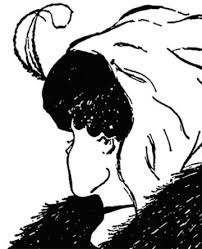
\includegraphics[width=\textwidth+\marginparsep+\marginparwidth]{./img/ovjv.png}\captionof{figure}{Oude vrouw jonge vrouw. \label{fig:ovjvFull}}
\end{adjustwidth}




\iffalse%=====wat een gelul
De tweede golf van de quantummechanica komt nauwelijks in het natuurkunde programma tot uiting. Het natuurkunde programma wordt in deze NLT module niet als bekend verondersteld. We behandelen wel de fysische principes die relevant zijn voor de module, enigszins vanwege de wens van de auteurs om quantumcomputing vanuit 'first principles' op te bouwen. 
Zonder deze inleiding zouden de belangrijke begrippen als \textit{superpositie}, \textit{verstrengeling}, \textit{interferentie} en \textit{meting} niet landen.
Deze begrippen komen in het natuurkunde programma trouwens niet voor. Grof gezegd beperkt het natuurkunde programma zich voornamelijk tot de zogenaamde eerste golf van de quantummechanica. Een respectabele keuze, maar ook in de natuurkundeles stellen leerlingen juist vragen over de onderwerpen die in deze module aan de orde komen. 

Het schrijven van deze module voor het vak NLT is een bijzondere uitdaging. Het brede spectrum van de achtergrond van leerlingen (de zachte en de harde beta's). 
We willen de kool en de geit sparen. we streven er naar om de 'wisA' leerligen binen boord te houden en de 'wisD' leerling een uitdaging te geven. Een uitdaging in differentiatie. 


Hoofdstuk 1 brengt ons de natuurkundige principes.
De belangrijke begrippen superpositie, verstrengeling interferentie en het meetprobleem komen aan de orde. We illustreren de begrippen zoveel mogelijk met experimenten. Er zijn veel meer ondersteunende experimenten dan we in de module kwijt kunnen. wellicht is er iets van uw gading bij op de ondersteuende website www.quantumrules.nl. 

Hoofdstuk 6 behandelt de maatschappelijke aspecten van deze komende technologie.

localisatie kenniscentrums Amsterdam, Delft Twente Eindhoven en theoretische groepen in Leiden, Groningen, [ref ]

We hopen met deze moduleleerlingen te interesseren voor de opleidingen 


skipistes

Het lukt ons niet een dun boekje te maken. De reader is meer dan 90 pagina's dik. Er zijn zijpaden opgenomen die niet allemaal bewandeld hoeven te worden. Natuurlijk ook niet printen. het leerlingen materiaal heeft augmented learning features waarmee de referenties prima te benaderen zijn vanuit je telefoon.
\fi%=====wat een gelul
\iffalse%=== nog meer gelul
\paragraph{Een didactische uitdaging} Het meeste beschikbare onderwijsmateriaal richt zich op de wisB leerlingen [refs]. natuurijk is het belangrijk om deze leerlingen  een carri\`erepad schetsen. Vectoralgebra, bases van eigenvectoren eigenwaarden, complexe getallen. Het domein van wiskunde B. Met deze begrippen kan de taal van quantumcomputing makkelijk worden ingeleid. De meeste tekstboeken behandelen hermitische en unitaire matrices, en de Bloch bol. Veel bestaande methoden zijn daarmee afgeleid van undergraduate courses, waarin een formele opbouw didactisch verandetowoord is. Er zijn twee versterkende redenen die deze keuze verantwoord maakt. Het publiek is geselecteerd, is een jaartje ouder en heeft daarmee een jaartje meer wiskunde in de pocket. Er is echter een veeel grotere trgroep ddie dan de aandacht ontsnapt. Het is belangrrijk juist deze leerligne bij de les te houden. Voor hetn is het mogelijk de latste keer dat ze met QC te maken krijgen. Dit is dus de enige kans een positieve ervaring aan hen mee te geven.
het is een stevige uitdaging deze twee doelen te bereiken. Gevaar in een spagaat terecht tekomen, en beide doelen te missen.
Wij streven ernaar deze module te schrijven voor alle leerlingen leerlingen die NLT volgen, dus ook voor de leerlingen met wisA in het pakket. Zij zoeken geen uitdaging in de lineaire algebra. Zonder wiskunde is QC echter niet te begrijpen. Als we te lang stil zouden staan bij de opbouw van het wiskundig formalisme, dan zouden we nooit een bevredigend einddoel kunnen halen. Dit dilemma tussen diepgang en haalbaar einddoel heeft de auteurs lang bezig gehouden. Wij vonden de oplossing door de module in twee\"en te splitsen. In het eerste klassikale deel wordt de wiskunde opgebouwd waarmee een minimaal quantumalgoritme begrepen kan worden. Dit algoritme is uniek voor een QC; het kan per se niet op een klassieke computer worden uitgevoerd. Dit klassiekale deel omvat ook andere aspecten zoals hardware, wat anticipaties over de maatschappelijke gevolgen voor het geval deze technologie doorzet, economie, ethiek. Het onderdeel wordt afgesloten met een toets. 
 


In het tweede deel van de cursus komt het open karakter van NLT goed tot uitintg.  kan gebruikt worden om te differenti\"eren. QC is een rijk onderwerp. We kunnen veel meer aanbieden dan we kwijt kunnen. enkele keuze modules worden nu bijgeleverd, maar het ligt in de bedoeling dat de verschillende kenniscentra in Nederland hiervoor in de toekomst bijdragen kunnen leveren.

\hrefqr{https://youtu.be/EmNQuK-E0kI}{What is the Quantum wave function, exactly?}
Brilliant 11:58 : Working out answers to problems is the only way you will ever gt a deeper understanding of this weird and wonderful piece of physics.

referentie aan Dr physics A


Een van de voordelen van het schrijven in latex is dat het document gecompileered kan worden in verschillende versies. Zo bestaat de leerlingenhandleiding bestaat in twee versies: een docentenexemplaar  met antwoorden in de marge dat ook als antwoordenboekje kan dienen,   en een zonder. Ook de diagnostische toets kan eenvoudig met en zonder antwoorden worden afgedrukt.

De documentatie van deze module is geschreven in Latex. Deze professionele opmaakomgeving maakt het makkelijker om wiskundige formules weer te geven. 
We leveren de pdf versie op, maar de bron code is beschikbaar voor docenten.
Er zijn diverse online converters van pdf naar doc. 
Een serieuze aanpak is \hrefqr{https://pandoc.org/}{Pandoc}. Pandoc streeft ernaar een universele document converter, dis ook  vanuit latex of pdf naar word te converteren. Het is wellicht makkelijker om latex te installeren.
\fi%== nog meer gelul

\tagged{eruit}{%--++--
\begin{enumerate}

\item 
\begin{flushleft}
\begin{minipage}{\textwidth}
\begin{tabular}{|r|c|c|c|}
\hline
                 & $q_{0}=\ket{0}$           & $q_{0}=\ket{1}$        &  \\ \hline
$q_{1}=\ket{0}$  & $\tfrac{1}{2}\alpha^2$    & $\tfrac{1}{2}\alpha^2$  & 
$\alpha^2$ \\ \hline
$q_{1}=\ket{1}$  & $\tfrac{1}{2}\beta^2$     & $\tfrac{1}{2}\beta^2$ & $\beta^2$  \\ \hline
                 & $\tfrac{1}{2}\left(\alpha^2+\beta^2\right)$     & $\tfrac{1}{2}\left(\alpha^2+\beta^2\right)$     & $\alpha^2+\beta^2$  \\ \hline
\end{tabular}
\end{minipage}%
\end{flushleft}

\item 
$\port{H}\ket{0}\port{Ryxx}\ket{0}=$\\
$\tfrac{1}{\sqrt{2}}\left(\ket{0}+\ket{1}\right)\port{Ryxx}\ket{0}=$\\
$\tfrac{1}{\sqrt{2}}\left(\ket{0}+\ket{1}\right)\left(\alpha\ket{0}+\beta\ket{1}\right)=$\\
$\tfrac{1}{\sqrt{2}}\alpha\ket{00}+\tfrac{1}{\sqrt{2}}\beta\ket{01}+
 \tfrac{1}{\sqrt{2}}\beta\ket{10}+\tfrac{1}{\sqrt{2}}\alpha\ket{11}$

\item 
\begin{flushleft}
\begin{minipage}{\textwidth}
\begin{tabular}{|r|c|c|c|}
\hline
         & $q_{0}=\ket{0}$ & $q_{0}=\ket{1}$ &  \\ \hline
$q_{1}=\ket{0}$  & $\tfrac{1}{2}\alpha^2$    & $\tfrac{1}{2}\beta^2$ &
$\tfrac{1}{2}\left(\alpha^2+\beta^2\right)$ 
\\ \hline
$q_{1}=\ket{1}$  & $\tfrac{1}{2}\beta^2$    & $\tfrac{1}{2}\alpha^2$ & $\tfrac{1}{2}\left(\alpha^2+\beta^2\right)$  \\ \hline
         & $\tfrac{1}{2}\left(\alpha^2+\beta^2\right)$     & $\tfrac{1}{2}\left(\alpha^2+\beta^2\right)$     & $\alpha^2+\beta^2$  \\ \hline
\end{tabular}
\end{minipage}%
\end{flushleft}

\item Als $q_0$ en $q_1$ niet verstrengeld zijn zijn het 'eerlijke muntjes'; de kansen zijn onafhankelijk. 
Uit vakje rechtsonder blijkt: $\alpha^2 + \beta^2=1$,\\
Uit de vier cellen met realisaties blijkt (op vier manieren) $\alpha^2 = \beta^2$, 
Opl: $\alpha = \pm\tfrac{1}{2},\beta = \pm\tfrac{1}{2}$ 
(We gebruiken geen complexe getallen)

\end{enumerate}
}%--++--

\end{document}
